%!TEX root = ../phd-thesis-lei-ma.tex

\chapter{\label{chap:collective}Collective Neutrino Oscillations}

Neutrino oscillations in the matter background have well defined linear dynamics as I  have discussed in the preceding chapters. In this chapter, I will discuss neutrino oscillations in a dense neutrino medium where the equation of motion becomes nonlinear.
%However, the universe provides many other much more exciting labs for neutrino physics.
One of such examples is the (core-collapse) supernova explosion which releases approximately $10^{58}$ neutrinos within seconds~\cite{Bahcall1987}. The neutrino density inside a supernova can be so large that that the neutrino self-interaction potential $H_{\nu\nu}$ to be comparable to or even larger than the matter potential in certain regions~\cite{Flowers1976a}. It has been shown that the self-interaction between the neutrinos can cause the neutrino medium to oscillate collectively~\cite{Duan2010, Duan2006}. The neutrino self-interaction also introduces a new characteristic energy scale which is proportional to the neutrino number density. As a result it is possible that neutrinos can oscillate on distance scales much shorter than the vacuum neutrino oscillation wavelength~\cite{Sawyer2016,Chakraborty2016}.
%~\cite{Malkus2014, Vaananen2015, Wu2015}.

In this chapter, I will first review some of the general features of collective neutrino oscillations and introduce the method of linearized flavor stability analysis. I will then discuss the dispersion relations of the collective modes of neutrino oscillations and show that it may or may not be related to the flavor stability of neutrino gas. Finally, I will demonstrate a preliminary study of a toy model which can be used to understand the neutrino oscillations in the presence of the neutrino halo~\cite{Sarikas2012a,Cherry2012}.
% review the neutrino collective oscillations and fast modes in neutrino collective oscillations. I will also review the connection between fast modes and dispersion relations proposed by I. Izaguirre et al~\cite{Izaguirre2016a}. Then I will show that the relation dispersion relations and fast modes is not well established. In the last few sections, I will discuss the neutrino halo problem, where scattering of neutrinos is considered.


% \section{\label{chap:collective-sec:collective}Collective Oscillations}


% \section{\label{chap:collective-sec:synchronization}Synchronization in Neutrino Oscillations}
% \section{\label{chap:collective-sec:collective}Collective Oscillations}
\section{Equation of Motion}

The equation of motion for neutrino oscillations with self-interaction is~\cite{Sigl1993}
\begin{equation}
   \ri \frac{\dd}{\dd t}\rho = [ \mathsf H,\rho],
   \label{chap:collective-sec:collective-eqn:equation-of-motion-general}
\end{equation}
where the total derivative is
\begin{equation}
   \frac{\dd}{\dd t} = \partial_t + \mathbf v\cdot \boldsymbol{\nabla},
\end{equation}
and the Hamiltonian is composed of three different terms:
\begin{equation}
   \mathsf H = \mathsf H_{\mathrm v} + \mathsf H_{\mathrm m} +\mathsf  H_{\nu\nu}.
\end{equation}
% \begin{equation}
%     \frac{d}{dt} = \frac{d}{dr},
%  \end{equation}
%  where $r$ is the distance travelled by the neutrino. A more general approach is to rewrite the total derivative
In the above equation, the vacuum Hamiltonian is
%$\mathsf H_\vv$, $\mathsf H_\mm$ and $\mathsf H_{\nu\nu}$ represents the vacuum Hamiltonian, matter potential, and neutrino self-interaction potential:
\begin{align*}
    \mathsf H_\vv =& \begin{cases}
    -\frac{1}{2}\eta \omega_\vv \sigma_3 & \text{for neutrinos},\\
    \frac{1}{2}\eta \omega_\vv \sigma_3 & \text{for antineutrinos},
    \end{cases}
\end{align*}
and the matter potential is
\begin{equation}
    \mathsf H_\mm = \frac{1}{2} \lambda \sigma_3  = \frac{1}{2} \sqrt{2}G_{\mathrm F} n_{\mathrm e} \sigma_3,
\end{equation}
where $\eta = +1$ for the normal neutrino mass hierarchy and $-1$ for the inverted neutrino mass hierarchy, $\omega_\vv$ is the vacuum oscillation frequency of the neutrino or antineutrino, and $n_{\mathrm e}$ is the net electron number density. The neutrino self-interaction is more complicated and can be written as
\begin{equation}
    \mathsf H_{\nu\nu} = \sqrt{2}G_{\mathrm F} \int \dd E' \dd\Omega_{\mathbf v'} \left[ n(E',\mathbf v')\rho(E',\mathbf v') - \bar n(E',\mathbf v')\bar\rho(E',\mathbf v') \right] (1-\mathbf v \cdot \mathbf v'),
    \label{chap:collective-sec:collective-eqn:equation-of-motion-self-interaction}
\end{equation}
where $n(E,\mathbf v)$ and $\rho(E, \mathbf v)$ are the number density and the flavor density matrix of the neutrino with energy $E$ and velocity $\mathbf v$, and $\bar n(E, \mathbf v)$ and $\bar \rho(E,\mathbf v)$ are the corresponding quantities of the antineutrino.
% \begin{align}
%     \mathsf H_\vv =& -\frac{1}{2}\beta\eta \omega_0 \sigma_3\\
%     \mathsf H_\mm =& \frac{1}{2} \sqrt{2}G_F n_e \sigma_3 \\
%     \mathsf H_{\nu\nu} =& \sqrt{2}G_F \int d\omega d\Omega_{\mathbf v'} n(\omega,\mathbf v')\beta(\mathbf v')\rho(\omega,\mathbf v') (1-\mathbf v \cdot \mathbf v').
% \end{align}
% I use $\eta=\pm 1$ for Normal Hierarchy and Inverted Hierarchy respectively. I also use $\beta=1$ for neutrinos and $\beta=-1$ for antineutrinos. In other words, the vacuum frequency is $\omega_\vv = \eta \omega_0$. $\beta(\mathbf v')$ indicates whether the density matrix $\rho(\omega,\mathbf v')$ is for neutrinos or antineutrinos. If $\beta(\mathbf v')=-1$, $\rho(\omega,\mathbf v')$ is for antineutrinos, vice versa. More explicitly, the vacuum Hamiltonian is
% \begin{align*}
%    \mathsf H_\vv =& \begin{cases}
%    -\frac{1}{2}\eta \omega_\vv \sigma_3 & \text{for neutrinos}\\
%    \frac{1}{2}\eta \omega_\vv \sigma_3 & \text{for antineutrinos}
%    \end{cases}
% \end{align*}
% while the neutrino-neutrino interaction Hamiltonian is
% \begin{align*}
%    \mathsf H_{\nu\nu} =& %\begin{cases}
%    \sqrt{2}G_{\mathrm F} \int d\omega d\Omega_{\mathbf v'} n(\omega,\mathbf v')\rho(\omega,\mathbf v') (1-\mathbf v \cdot \mathbf v') & \text{interacting with neutrinos} \\
%    - \sqrt{2}G_{\mathrm F} \int d\omega d\Omega_{\mathbf v'} n(\omega,\mathbf v')\bar\rho(\omega,\mathbf v') (1-\mathbf v \cdot \mathbf v') &  \text{interacting with antineutrinos}
% %    \end{cases}
% \end{align*}

% Please note that I have used the following notation.
% \begin{itemize}
%     \item $\omega_\vv$ is the absolute value of the frequency, since $\eta$ takes care of the signs;
%     \item The integral in $\mathsf H_{\nu\nu}$ must take care of both interactions with neutrinos and anti-neutrinos.
% \end{itemize}
% I also use the following quantities in this chapter.
% \begin{itemize}
%     \item $\lambda$ is the same as the previous chapter
%     \begin{equation}
%         \lambda = \sqrt{2} G_{\mathrm F} n_{\mathrm e}.
%     \end{equation}
% \item Angle distribution of number density is denoted as
% \begin{equation}
%     f(\mathbf v) = \frac{n(\omega,\mathbf v)}{n_{\mathrm{t}}},
% \end{equation}
%    where $n_{\mathrm{total}}$ is the total number density of neutrinos for all energies. It can also be defined for anti-neutrinos
% \begin{equation}
%       \bar f(\mathbf v) = \frac{\bar n(\omega,\mathbf v)}{\bar n_{\mathrm{t}}},
% \end{equation}
% where $\bar n_{\mathrm{t}}$ is the total number density of antineutrinos. One of the useful models is the line model, where neutrinos are emitted from a line. This model is a 2D neutrino problem. The direction of momentum $\mathbf v$ only depends on one angle, hence the distribution becomes $f(\theta)$. With this definition, the number density of neutrinos for some specific frequency $\omega$ within a range of angle $[\theta, \theta + d\theta]$ can be calculated using
% \begin{equation}
%       n_{\mathrm{t}} f(\theta) d\theta.
% \end{equation}
% Similarly, the the number density of antineutrinos within angle $[\theta,\theta+d\theta]$ is
% \begin{equation}
%     \bar n_{\mathrm{t}} \bar f(\theta) d\theta.
% \end{equation}
% \item An asymmetry parameter can be defined to connect the total number density of neutrinos and antineutrinos,
% \begin{equation}
%     \alpha = \frac{\bar n_{\mathrm{t}} }{n_{\mathrm{t}}}.
% \end{equation}

% \end{itemize}

% With the three definitions we simplify the neutrino self-interactions with matter effect
% \begin{align*}
%     \mathsf H_\mm =& \frac{1}{2} \lambda \sigma_3 \\
%     \mathsf H_{\nu\nu} =& \sqrt{2}G_{\mathrm F} n_{\mathrm{t}} \int d\omega d\Omega_{\mathbf v'} f(\omega,\mathbf v)\rho(\omega,\mathbf v') (1-\mathbf v \cdot \mathbf v') \\
%    & - \sqrt{2}G_{\mathrm F} \bar n_{\mathrm{t}} \int d\omega d\Omega_{\mathbf v'} \bar f(\omega,\mathbf v)\bar\rho(\omega,\mathbf v') (1-\mathbf v \cdot \mathbf v') \\
%    =& \frac{1}{2}\mu \int d\omega d\Omega_{\mathbf v'} f(\omega, \mathbf v)\rho(\omega,\mathbf v') (1-\mathbf v \cdot \mathbf v') \\
%    & - \frac{1}{2}\alpha \mu \int d\omega d\Omega_{\mathbf v'} \bar f(\omega, \mathbf v)\bar\rho(\omega,\mathbf v') (1-\mathbf v \cdot \mathbf v') ,
% \end{align*}
% where
% \begin{equation}
%    \mu = 2\sqrt{2} G_{\mathrm F} n_{\mathrm{t}}.
% \end{equation}

The presence of the neutrino self-interaction potential makes the equation of motion \ref{chap:collective-sec:collective-eqn:equation-of-motion-general} nonlinear, and many interesting phenomena arise because of it. For example, a dense neutrino medium can experience synchronized oscillations during which all the neutrinos and antineutrinos oscillate with the same frequency~\cite{Pastor2002,Hannestad2006,Raffelt2008,Duan2010}. To see this, I will consider an isotropic and homogeneous neutrino gas and use the flavor isospin picture discussed in Sec.~\ref{chap:basics-sec:flavor-isospin-pic}. The flavor isospin of the neutrino is defined by
% With the equation of motion Eqn.~\eqref{chap:collective-sec:collective-eqn:equation-of-motion-general}, many aspects of such a system can be explored, such as neutrino bulb model, line model, etc. New dynamics, such as spectral split, synchronizations, matter-neutrino resonances, have been identified~\cite{Duan2006,Malkus2014,Vaananen2015}. Synchronization is one of the most surprising results which might happen when neutrino number density is large.
\begin{equation}
   \rho = \frac{1}{2} + \vec s \cdot \vec \sigma.
\end{equation}
% and that of the antineutrino is defined by
% \begin{equation}
%     \bar\rho = \frac{1}{2} - \vec s \cdot \vec \sigma.
% \end{equation}
% The reason for the negative sign in the above definition for the antineutrino is due to the sign in front of $\bar \rho(E, \mathbf v)$ in Eqn.~\eqref{chap:collective-sec:collective-eqn:equation-of-motion-self-interaction}.
The equation of motion of the flavor isospin is
\begin{equation}
    \dot{\vec s} = \vec s \times \left(\vec H_\vv + \vec H_{\nu\nu} \right),
    \label{chap:collective-eqn:flavor-isospin-eom}
\end{equation}
where
\begin{equation}
   \vec H_{\mathrm v} =  \omega_{\mathrm v}\begin{pmatrix}
   -\sin 2\theta_{\mathrm v}\\
   0 \\
   \cos 2\theta_{\mathrm v}
   \end{pmatrix} = \omega_\vv \vec B,
\end{equation}
and
\begin{equation}
\vec H_{\nu\nu} = \sqrt{2}G_{\mathrm F} \int \dd E' n(E') \vec s(E').
\end{equation}
Here for simplicity I have assumed $n_{\mathrm e}=0$ and $\bar n=0$. When the neutrino density is very large, $\vec H_{\nu\nu}$ dominates over $\vec H_\vv$ in Eqn.~\eqref{chap:collective-eqn:flavor-isospin-eom}, and $\vec s_\vv$ precesses about $\vec H_{\nu\nu}$ rapidly. Meanwhile, the total flavor isospin
\begin{equation}
    \vec S = \int \dd E' f(E') \vec s(E')
\end{equation}
precesses about $\vec H_\vv$ slowly with a mean oscillation frequency $\langle \omega_\vv \rangle$, where
\begin{equation}
    f(E) = \frac{ n(E) }{ \int \dd E' n(E') }
\end{equation}
is the energy distribution of the neutrino. To see this, one can multiply Eqn.~\eqref{chap:collective-eqn:flavor-isospin-eom} by $f(E)$ and integrate over $E$ which gives
\begin{align}
    \dot{\vec S} &= \int \dd E f(E)\vec s(E) \times \omega_\vv \vec B \\
    &\to \int \dd E f(E) \left[ \frac{\vec s(E) \cdot \vec S}{ \lvert \vec S \rvert^2 } \vec S \right] \times \omega_\vv \vec B \\
    &= \langle \omega_\vv \rangle \vec S \times \vec B,
\end{align}
where
\begin{equation}
    \langle \omega_\vv \rangle  = \int \dd E f(E) \left[ \frac{\vec s(E) \cdot \vec S}{ \lvert \vec S \rvert^2 } \right] \omega_\vv.
\end{equation}
In the above equation I have replaced flavor isospin $\vec s$ with its projection along the direction of $\vec S$ because its precession about $\vec S$ is much faster than the precession of $\vec S$ about $\vec B$.

% But the neutrino coherent scattering term requires some simplifications. For the purpose of the physics picture, we consider isotropic and homogeneous model composed of neutrinos only which leads to
% \begin{equation}
%    \vec H_{\nu\nu} = \sqrt{2}G_{\mathrm F} n_\nu \int d\vec p'^3 (1-\vec p \cdot \vec p') (\rho_{\vec p'} - \bar\rho_{\vec p'}) = \sqrt{2}G_{\mathrm F} n_\nu \int dE' \frac{1}{n_\nu}(\rho_{E'} - \bar\rho_{E'}).
%    \label{chap:collective-sec:collective-eqn:isotropic-homogeneous-self-interaction}
% \end{equation}
% The flavor isospin will precess around $\vec H_{\nu\nu}$ assuming no vacuum or matter contributions.%, as shown in Fig.~\ref{chap:collective-sec:collective-fig:self-interaction}.
% We have to define a vector, which is an integral of flavor-isospin vector over all energies or frequencies,
% \begin{equation}
%    \vec D = \int d\omega' \vec s(\omega').
% \end{equation}
% Eqn.~\eqref{chap:collective-sec:collective-eqn:isotropic-homogeneous-self-interaction} becomes $\vec H_{\nu\nu} = \mu \vec D$, where $\mu = \sqrt{2}G_{\mathrm F} n_\nu$.

% \begin{figure}[h!tbp]
%     \centering
%     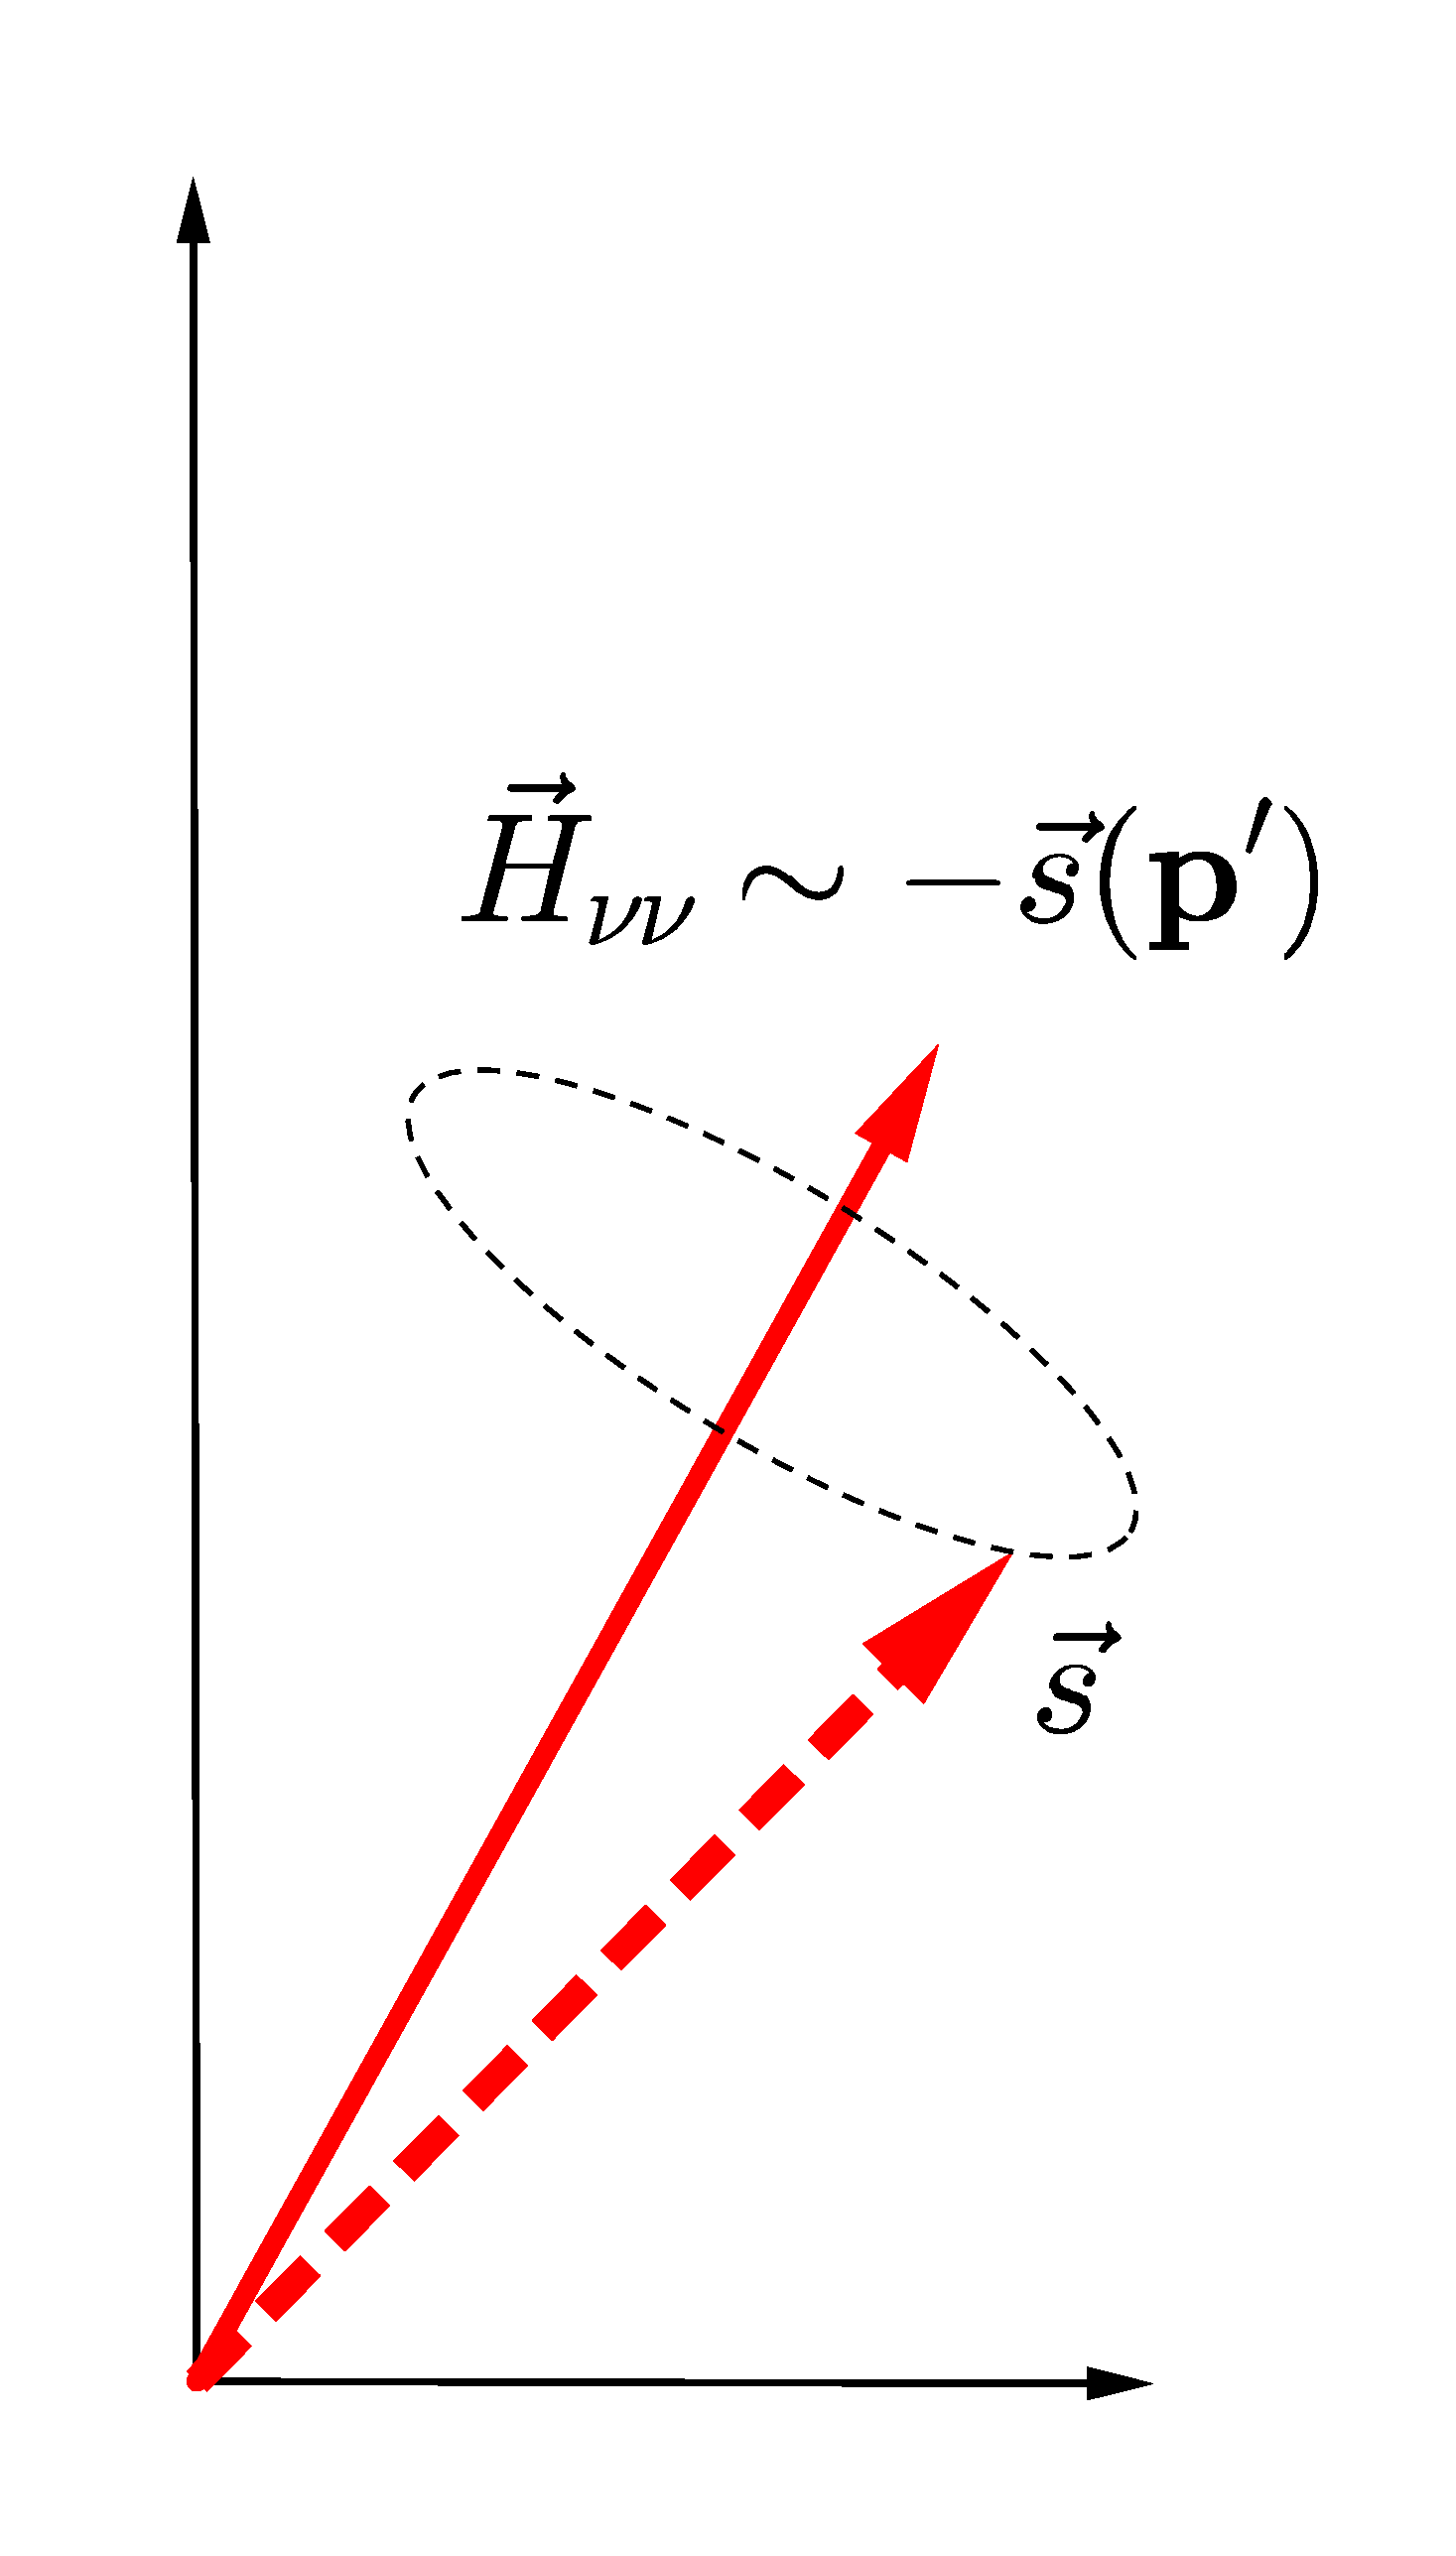
\includegraphics[width=0.4\textwidth]{chapters/assets/matter/self-interaction}
%     \caption{ Flavor isospin $\vec s$ precess around the Hamiltonian $\vec H_{\nu\nu}$ in flavor isospin space.}
%     \label{chap:collective-sec:collective-fig:self-interaction}
%  \end{figure}


% For single energy or flavor isospins aligned in the same direction, this vector is in the direction of the flavor isospin vector. If the flavor isospins are initially prepared in completely random and uniformly distributed directions, $\vec D\sim 0$.

% Synchronization occurs when the neutrino number density becomes large. $\vec D$ will wobble around very fast due to the precessions of flavor isospins, but almost stays in one direction. All the spins precess with the same frequency which is determined by $\mu$.

% With vacuum contribution $\vec H_{\mathrm v}$ and matter contribution $\vec H_{\mathrm m}$ to the Hamiltonian, we expect $\vec D$ to precess around $\vec H_{\mathrm v} + H_{\mathrm v}$, if the precession frequency of flavor isospins around $\vec D$ is much larger than the precession frequency of $\vec D$ around  $\vec H_{\mathrm v} + H_{\mathrm v}$.



\section{\label{chap:collective-sec:two-beams}Two-Beam Model and Flavor Instabilities}

During the synchronized flavor transformation, the whole neutrino medium behaves as if there was a single neutrino oscillating with the mean frequency $\langle \omega_\vv \rangle$ in vacuum. Under certain conditions, the neutrino self-interaction potential can cause the neutrino medium to evolve in a way completely different than the vacuum oscillations. I will illustrate this phenomenon using the two-beam neutrino model.

In the two-beam model, neutrinos and antineutrinos are emitted in two different directions from a plane which we assume to be the $x$-$y$ plane. I define the emission angles of the neutrino beams $\theta_1$ and $\theta_2$ inside the plane spanned by the velocity vectors of the two neutrino beams (see Fig.~\ref{chap:collective-sec:two-beams-fig:two-beam-line-model}). I will assume that the neutrino emission plane is homogeneous and that the neutrino and antineutrino have the same density $n$ in the emission plane. I will also assume that the matter density vanishes everywhere in space.



\begin{figure}[!htbp]
    \centering
    % 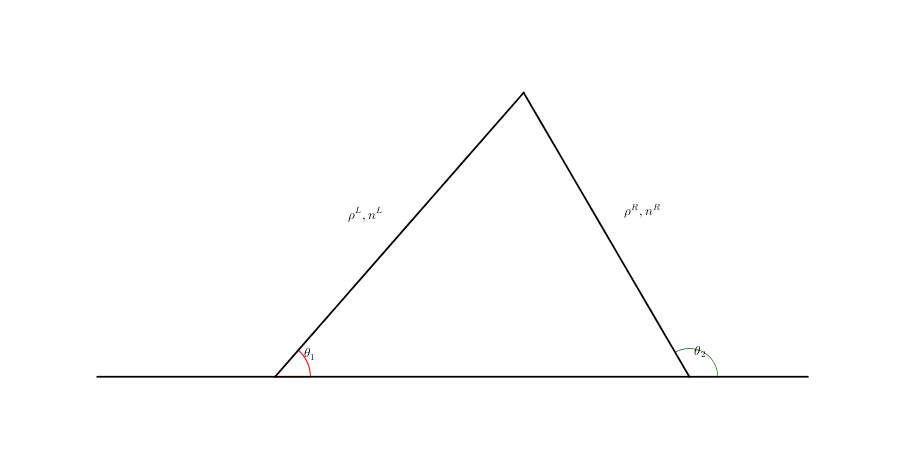
\includegraphics[width=\textwidth]{chapters/assets/dr/two-beam-line-model}
    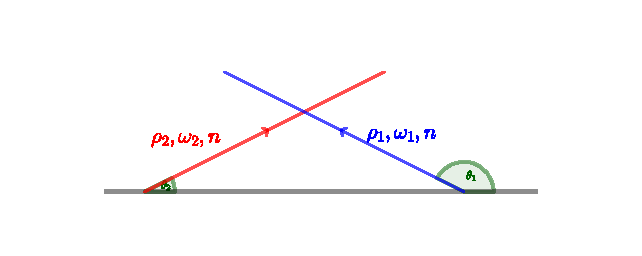
\includegraphics[width=\textwidth]{chapters/assets/collective/two-beams-model-sym}
    \caption{The geometry of two-beam model. The $i$th ($i=1,2$) neutrino beam has emission angle $\theta_i$, vacuum oscillation frequency $\omega_i$ and density matrix $\rho_i$. Both neutrino beams have the same number flux $n$.}
    \label{chap:collective-sec:two-beams-fig:two-beam-line-model}
\end{figure}


The Hamiltonian of the $i$th neutrino beam in the vacuum basis is
\begin{align}
   \mathsf H_i &= -\frac{\omega_i}{2}  \sigma_3 + \mu ( \rho_1 -  \rho_2),
\end{align}
where $\omega_1 = \eta\omega_\vv$ for the neutrino beam and $\omega_2=-\eta\omega_\vv$ for the antineutrino beam,
\begin{align}
   \mu = \sqrt{2} G_{\mathrm F}  (1 - \cos(\theta_1 - \theta_2))  n
\end{align}
is the neutrino self-interaction potential.

I will assume that the neutrino and antineutrino are emitted in the pure electron flavor at $z=0$. I will also assume the vacuum mixing angle $\theta_\vv \ll 1$. Therefore, the flavor density matrix of the $i$th neutrino beam in the vacuum basis at $z=0$ is
\begin{equation}
    \rho_i (z=0)  \approx  \begin{pmatrix}
        1 & \epsilon_i (0) \\
        \epsilon_i^* (0) & 0
    \end{pmatrix},
    \label{chap:collective-sec:two-beams-eqn:density-matrix-perturbed}
\end{equation}
where
\begin{equation}
    \epsilon_i(0) = \sin (2\theta_\vv) \ll 1.
\end{equation}

I solve the two-beam model numerically with $\epsilon_i = 10^{-3}$ and $\eta=-1$. The solution is shown in Fig.~\ref{chap:collective-sec:two-beams-fig:two-beam-line-model-numerical-solution}. When $\omega_\vv z \ll 1$, the flavor isospin of the neutrino stays in the electron flavor state, i.e., in the direction of third axis $\vec e_3$ in the flavor isospin space (see the left panel of Fig.~\ref{chap:collective-sec:two-beams-fig:two-beam-line-model-numerical-solution}). Accordingly, the electron flavor survival probability $P_{\nu_\ee}\approx 1$ at small $z$ but falls down rapidly at a certain value of $z$ (see the right panel of Fig.~\ref{chap:collective-sec:two-beams-fig:two-beam-line-model-numerical-solution}). Then both the flavor isospin and $P_{\nu_\ee}$ come back to their original positions until they fall down again. The flavor isospin of the antineutrino follows a similar pattern but is in a different direction. This flavor transformation phenomenon is clearly different from the vacuum oscillations shown in Fig.~\ref{chap:basics-section:neutrinos-fig:vacuum-2-flavor-osc}.

\begin{figure}[!htbp]
    \centering
    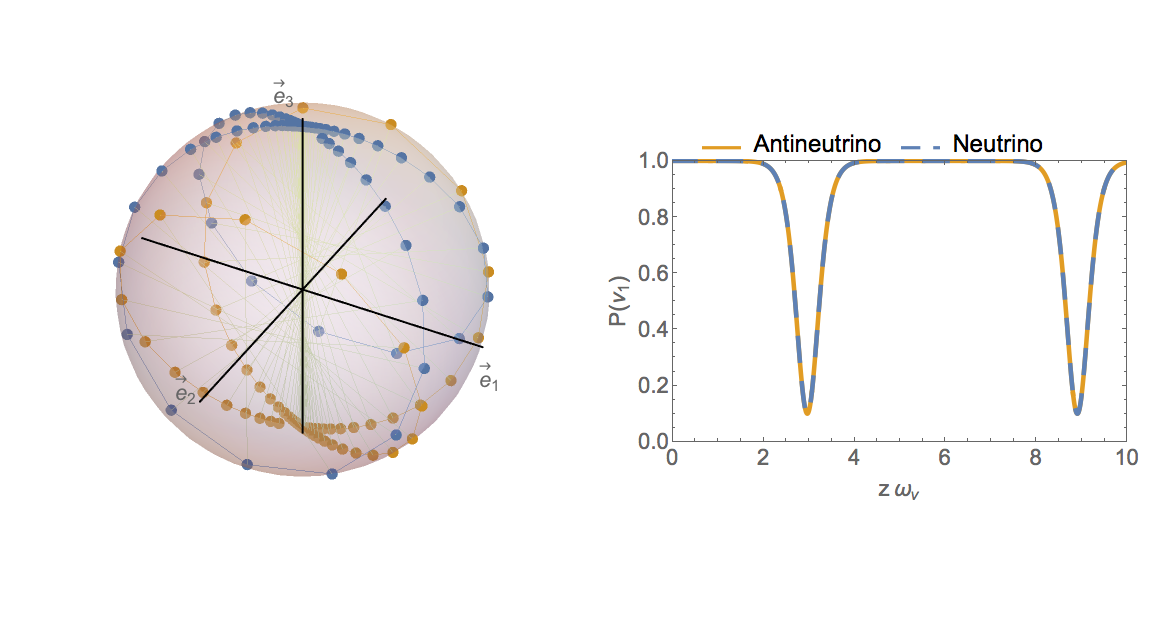
\includegraphics[width=\textwidth]{chapters/assets/collective/bipolar-animie100}
    \caption{The numerical solution to the two-beam model. The left panel shows the position of the flavor isospin of the neutrino beam (in blue) and the antineutrino beam (in orange). The right panel shows the probabilities as functions of distance $z$ (in unit of $\omega_\vv^{-1}$) for the neutrinos and antineutrinos to remain in the $\ket{\nu_1}$ and $\ket{\bar\nu_1}$ states, which are the same as the survival probabilities of the electron flavor when mixing angle $\theta_\vv \ll 1$. In this calculation, the emission angles are $\theta_1=5\pi/6$ and $\theta_2=\pi/6$, the neutrino self-interaction potential is $\mu=5 \omega_\vv$, and the neutrino mass hierarchy is inverted. }
    \label{chap:collective-sec:two-beams-fig:two-beam-line-model-numerical-solution}
\end{figure}

To gain a deeper understanding of the collective oscillation phenomenon, I will focus on the linear regime where $\lvert \epsilon_i(z) \rvert \ll 1$. The equation of motion is linearized in this regime and becomes
\begin{equation}
    \ri \partial_z \begin{pmatrix}
        \epsilon_1 \\
        \epsilon_2
    \end{pmatrix} =  \begin{pmatrix}
        \mu + \eta\omega_\vv & - \mu \\
        \mu & - \eta\omega_\vv - \mu
    \end{pmatrix} \begin{pmatrix}
        \epsilon_1 \\
        \epsilon_2
    \end{pmatrix}.
    \label{chap:collective-sec:bipolar-linearized-eom}
\end{equation}
This equation has two normal modes which corresponds to the collective modes of neutrino oscillations:
\begin{equation}
    \begin{pmatrix}
        \epsilon_1 (z) \\
        \epsilon_2 (z)
    \end{pmatrix} = \begin{pmatrix}
        Q_{1\pm} \\
        Q_{2\pm}
    \end{pmatrix} e^{i K_{z\pm} z},
    \label{chap:collective-sec:two-beams-eqn:equation-of-motion-collective-mode-assumption}
\end{equation}
where $(Q_{1\pm}, Q_{2\pm})^{\mathrm T}$ are the eigenvectors of the two normal modes, and
\begin{equation}
    K_{z\pm} = \pm \sqrt{ \omega_\vv (\omega_\vv + 2 \eta \mu) }
\end{equation}
are the wavenumbers of the corresponding modes. For the normal mass hierarchy, $\eta = 1$, and $K_{z\pm}$ are always real. In this case, the electron flavor probability $P_{\nu_\ee}$ is always approximately 1. However, for the inverted neutrino mass hierarchy, $\eta=-1$, and $K_{z\pm}$ are imaginary when $\mu > \omega_\vv/2$. The normal mode with wavenumber $K_{z-} = -\ri \sqrt{ \omega_\vv (2 \mu-\omega_\vv) }$ is a runaway solution which explains the rapid decrease of $P_{\nu_\ee}$ in Fig.~\ref{chap:collective-sec:two-beams-fig:two-beam-line-model-numerical-solution}.




% The linearized equation of motion becomes
% \small\begin{align}
%    &\ri \partial_z \begin{pmatrix}
%    \epsilon_1 \\
%    \epsilon_2
%    \end{pmatrix} =  - i \begin{pmatrix}\cot\theta_1\partial_x & 0 \\
%    0 & \cot\theta_2 \partial_x
%    \end{pmatrix} \begin{pmatrix}
%    \epsilon_1 \\
%    \epsilon_2
%    \end{pmatrix} + \nonumber\\
%    &
%    \frac{1}{2}\begin{pmatrix}
%    (\lambda+ \mu_2 - \eta \omega_1 - \mu_2 \cos(\theta_1-\theta_2) )/\sin \theta_1 & -\mu_2 (1-\cos(\theta_1-\theta_2)) /\sin \theta_1\\
%    -\mu_1 (1- \cos(\theta_1-\theta_2))/\sin\theta_2 & (\lambda + \mu_1 - \eta \omega_2 - \mu_1 \cos(\theta_1-\theta_2) )/\sin\theta_2
%    \end{pmatrix}\begin{pmatrix}
%    \epsilon_1 \\
%    \epsilon_2
%    \end{pmatrix},
%    \label{chap:collective-sec:two-beams-eqn:line-model-two-beams-all-neutrino-linearized-eom}
% \end{align}\normalsize
% where
% \begin{align*}
%    \mu_1 =& \sqrt{2}G_F n_{t,1}\\
%    \mu_2 =& \sqrt{2}G_F n_{t,2}.
% \end{align*}



% \subsection{Left-right Symmetric Emission}


% We first consider a simple case, where $\theta_1=\pi-\theta_2\equiv\theta$, $\lambda=0$, $\eta=1$, and homogeneous in $x$ direction. For simplicity we define
% \begin{align*}
%    \mu =& \sqrt{2}G_F (n_1 + n_2)\\
%    \mu_i =& \mu \frac{n_i}{n_1+n_2}\equiv \mu f_i \\
%    \xi = & 1-\cos(\theta_1-\theta_2) \\
%    \omega'_i = & \lambda - \eta\omega_i.
% \end{align*}

% % I am aware that this is not a self-consistent example since $\theta_1=\theta_2$ indicates that $\xi=0$. As we will see, no instability is present in this case. However, we keep the term $\xi$ because we need to analyze the effect of symmetry breaking. This example builds up a formalism.

% The equation for perturbations becomes
% \begin{equation}
%    i\partial_z\begin{pmatrix}
%    \epsilon_1 \\
%    \epsilon_2
%    \end{pmatrix} = \frac{1}{2\sin\theta} \begin{pmatrix}
%    \omega'_1 + \mu f_2\xi & -\mu f_2 \xi \\
%    -\mu f_1 \xi & \omega'_2 + \mu f_1 \xi
%    \end{pmatrix}\begin{pmatrix}
%    \epsilon_1 \\
%    \epsilon_2
%    \end{pmatrix}.
%    \label{eqn-linearized-eom-symmetric-eg}
% \end{equation}
% Since $\mu$ is the most important energy scale in this problem, we scale all energies with it.
% \begin{equation}
%    i\partial_{\hat z}\begin{pmatrix}
%    \epsilon_1 \\
%    \epsilon_2
%    \end{pmatrix} = \frac{1}{2\sin\theta} \begin{pmatrix}
%    \hat\omega'_1 +  f_2\xi & - f_2 \xi \\
%    - f_1 \xi & \hat\omega'_2 +  f_1 \xi
%    \end{pmatrix}\begin{pmatrix}
%    \epsilon_1 \\
%    \epsilon_2
%    \end{pmatrix},
% \end{equation}
% where
% \begin{align*}
%    \partial_{\hat z} =& \frac{d}{\mu dz} \\
%    \hat \omega'_i =& \frac{\omega'_i}{\mu}.
% \end{align*}


% The characteristic equation for this equation is
% \begin{equation}
%    \left( ( \Omega - \hat\omega'_1 - f_2\xi )(\Omega - \hat\omega'_2-f_1\xi) - f_1 f_2 \xi^2 \right) =0,
%    \label{chap:collective-sec:two-beams-eqn:two-beam-line-characteristic-eqn-simple}
% \end{equation}
% which is simplified to
% \begin{equation*}
%    (\Omega-\Omega_1)(\Omega-\Omega_2) -f_1f_2\xi^2 = 0,
% \end{equation*}
% where
% \begin{align*}
%    \Omega_1 = & \hat\omega'_1 + f_2 \xi\\
%    \Omega_2 = & \hat\omega'_2 + f_1 \xi.
% \end{align*}
% Complete the square
% \begin{equation*}
%    (\Omega - (\Omega_1 + \Omega_2)/2)^2 = \frac{1}{4}(\Omega_1-\Omega_2) + f_1f_2\xi^2.
% \end{equation*}
% The solution becomes
% \begin{equation}
%    \Omega = \frac{1}{2}(\Omega_1+\Omega_2)\pm\sqrt{ (\Omega_1-\Omega_2)^2/4 + f_1f_2\xi^2 }.
% \end{equation}
% The condition to have positive imaginary part is
% \begin{equation*}
%    (\Omega_1-\Omega_2)^2 + 4f_1f_2\xi^2 < 0,
% \end{equation*}
% or
% \begin{equation*}
%    -2\sqrt{-f_1f_2\xi^2}<\Omega_1-\Omega_2<2\sqrt{-f_1f_2\xi^2},
% \end{equation*}
% and $f_1f_2\xi^2<0$. Recall the meaning of $f_i$,
% \begin{equation*}
%    f_i = \frac{n_i}{n_1+n_2},
% \end{equation*}
% instability requires that we have a spectrum crossing, i.e., $n_1$ and $n_2$ have different signs. Plug in the definitions of $\Omega_i$,
% \begin{equation*}
%    -2\sqrt{-f_1f_2\xi^2}< \eta(- \omega_1 + \omega_2)/\mu + (f_2 - f_1)\xi < 2\sqrt{-f_1f_2\xi^2}.
% \end{equation*}
% From this we can infer
% \begin{itemize}
%     \item $f_1f_2$ has to be negative, which means we can NOT have instabilities with only neutrinos or antineutrinos with all the symmetries we assumed. This is crossing.

% \item $-\omega_1+\omega_2=0$ will remove the instability. So we have to have both neutrinos and antineutrinos.
% \item $f_2-f_1$, $\eta(\omega_2-\omega_1)$, and $\mu$ set limit on each other.
% \item $\theta_1=\theta_2\equiv \theta$ removes the instability since it leads to $\xi=0$. The emission has to be asymmetric in this simple two beams model. This is trivial since equal emission angle means the beams are not colliding.
% \end{itemize}


% % .. admonition:: But why?
% %   :class: warning

% %   We have these conclusions. But why?

% %   What are the roles of

% %   1. :math:`f_i`,
% %   2. neutrino beam and antineutrino beam,
% %   3. hierarchy,
% %   4. neutrino number density variations,
% %   5. variations of angular distributions of neutrinos,
% %   6. variations of energy spectrum of neutrinos.


% Another way of understanding this equation is to think of it as the growth of the length of the vector $\vec v = (\epsilon_1,\epsilon_2)^T$. For an arbitrary matrix differential equation of the form
% \begin{equation*}
%   \partial_z \mathbf v = \mathbf A \mathbf v,
% \end{equation*}
% we can always decompose the matrix $\mathbf A$ into symmetric part and skew-symmetric part
% \begin{equation*}
%   \mathbf A = \frac{1}{2}(\mathbf A + \mathbf A^T) + \frac{1}{2}(\mathbf A - \mathbf A^T) \equiv \mathbf A^+ + \mathbf A^-.
% \end{equation*}
% We can identify the effect of $f_1-f_2$ but this is not particularly useful since we can not say anything about the eigenvalues of matrix $\mathbf A$ from the eigenvalues of matrix $\mathbf A^+$ and $\mathbf A^-$.



% \subsection{Breaking Symmetries}



% For a line model, the symmetries we have are
% \begin{itemize}
%     \item Time translation symmetry;
% \item Translation symmetry along the line;
% \item Energy spectrum of the beams; One of particular interest is to have different neutrino spheres for different energies which can be investigated using two beam model.
% \item Number density of left and right beams;
% \item Angle of left and right beams;
% \item With and without matter.
% \item Similar to the discussion of varying matter potential, symmetries can be broken globally, i.e., distribution as a function of spacetime coordinates.
% \end{itemize}

% I will discuss some of the symmetries mentioned above.



% \subsubsection{Emission Angle Parity Symmetry}

% The emission angles change the value of $\xi=1-\cos(\theta_1-\theta_2)$ as well as rescale the quantities by angle dependent factor $1/\sin\theta_i$.

% To see the importance of angles, we can redefine some quantities
% \begin{align*}
%    \omega''_i=& \frac{\omega'_i}{\sin\theta_i}\\
%    f''_1=&\frac{f_1}{\sin\theta_2} \\
%    f''_2=&\frac{f_2}{\sin\theta_1}.
% \end{align*}
% The we will reach the same characteristic equation as Eqn. \ref{chap:collective-sec:two-beams-eqn:two-beam-line-characteristic-eqn-simple}. So the angles serves as shift of energy gap and angular distribution.

% The region of instability changes in a convoluted way. Given angles we can always write down the expression and find out.
% \begin{itemize}
%     \item  The criteria of existence of instability doesn't change.
% \item  The region of instability changes.
% \end{itemize}


% \subsubsection{Matter Effect}


% Including matter will define vacuum frequencies, $\omega'_i$, which is effectively just a shift of vacuum frequencies. In the symmetric emission case, $\omega'_1-\omega'_2$ is independent of matter effect. But breaking the emission symmetry generates the degeneracy,
% \begin{equation}
%    \hat\omega''_1-\hat\omega''_2=( \lambda/\sin\theta_1 - \lambda/\sin\theta_2 + \eta(- \omega_1/\sin\theta_1 + \omega_2/\sin\theta_2) )/\mu`.
% \end{equation}

% We notice that very large matter density shift the region to very small $\mu$.

% However, matter effect is not always this simple. Suppose we have different matter potential for different beams, when they collide they would have built a different phase due to matter effect.

% The inhomogeneous matter effect has been studied in \cite{Mangano2014}. It can excite high Fourier moments of flavor-isospin picture, which makes a lot of sense because it generates fine structure in the x direction. This might be integrated into LESA effect.



% \subsubsection{Translation Symmetry}


% Translation symmetry is better explained by introducing Fourier transform in x direction.

% For each mode, a term that is proportional to Fourier mode index $m$. It only appears in diagonal elements, thus is effectively a shift of vacuum frequencies, thus energies of neutrinos.

% For each Fourier mode
% \begin{equation*}
%    \begin{pmatrix}
%    \epsilon_1 \\
%    \epsilon_2
%    \end{pmatrix} =  \mathbf Q(\Omega,k) e^{-i(\Omega t- k x)},
% \end{equation*}
% where we set $\Omega=0$.

% First term in RHS of Eqn.~ \ref{chap:collective-sec:two-beams-eqn:line-model-two-beams-all-neutrino-linearized-eom} becomes
% \begin{equation*}
%    - i \begin{pmatrix}\cot\theta_1\partial_x & 0 \\
%    0 & \cot\theta_2 \partial_x
%    \end{pmatrix} \begin{pmatrix}
%    \epsilon_1 \\
%    \epsilon_2
%    \end{pmatrix} = k \begin{pmatrix}\cot\theta_1 & 0 \\
%    0 & \cot\theta_2
%    \end{pmatrix} \begin{pmatrix}
%    Q_1 \\
%    Q_2
%    \end{pmatrix}.
% \end{equation*}
% We now define $\hat\omega''_i$, so that
% \begin{equation*}
%    \hat\omega''_{k,i} = \hat \omega''_i + 2\hat k\cot\theta_i,
% \end{equation*}
% where $\hat k=k/\mu$.

% The $k$ term contributes to the difference between $\Omega_{k,i}\equiv \hat\omega''_{k,i}+ f''_i\xi$.

% We notice that instability criteria doesn't change. However, the regime of instability changes. We also know that the instability region is determined by
% \begin{equation}
%    \lvert \Delta\hat\omega''_{12} + 2\hat k (\cot \theta_1 - \cot\theta_2) + \Delta f''_{12}\xi \rvert < \sqrt{-f_1f_2\xi^2},
% \end{equation}
% where $\Delta \hat \omega''_{12} = \hat\omega''_1-\hat\omega''_2$. The instability region shift from
% \begin{equation}
%    -\sqrt{-f''_1f''_2\xi^2} -\Delta f''_{12}\xi < (\Delta\omega''_{12} + 2 k(\cot\theta_1-\cot\theta_2))/\mu < \sqrt{-f''_1f''_2\xi^2} -\Delta f''_{12}\xi
% \end{equation}
% If $\lvert \Delta\omega''_{12} + 2 k(\cot\theta_1-\cot\theta_2) \rvert$ becomes larger, the region of instability is shifted to larger $\mu$, i.e., larger number density.



% \subsubsection{Number Density of Emission}


% A crossing is required to have instability, i.e., $-f''_1f''_2>0$. Meanwhile the number density on the left and right have little effects on the existence of instability. It shifts the region of instability for $\mu$.


% \subsubsection{Energy of Emission}



% Different energy of two beams will make sure $-\omega_1 + \omega_2\neq 0$. It has no effects on the criteria but changes the $\mu$ region of instability.


% % \subsubsection{Time Translation Symmetry}



% % .. admonition:: Time Translational Symmetry
% %   :class: warning

% %   How about time translational symmetry? I need to write down the equation of motion that is related to time.

% %   Two limits are of particular interest.

% %   1. Adiabatic limit,
% %   2. Super fast time variants.



% For completeness, I can also write down the linearized equation of motion without translational symmetries, c.f.~Eqn.~\eqref{chap:collective-sec:two-beams-eqn:line-model-two-beams-all-neutrino-linearized-eom}. I know that real symmetric matrix has only real eigenvalues, from which I infer that $\mu_1=\mu_2$ and $\theta_1=\theta_2$ removes the instability.
% For translation symmetric models, that is $\partial_x\to 0$, I have the eigenvalues
% \begin{equation*}
%    \Omega = \frac{1}{4}(A\pm B),
% \end{equation*}
% where
% \begin{align*}
%    A=& -\eta \omega_1/\sin\theta_1 - \mu_2 /\sin\theta_1 + \eta \omega_2 /\sin\theta_2 + \mu_1 \xi /\sin\theta_2 + \lambda(1/\sin\theta_1 + 1/\sin\theta_2)  \\
%    B=& \left(
%       -4[(\lambda-\eta\omega_1)(\lambda +\eta\omega_2) + (\lambda (\mu_1-\mu_2) -\eta (\mu_1\omega_1 + \mu_2\omega_2) )\xi ] \sin\theta_1 \sin\theta_2\right. \\
%       &\left.+ [(\lambda + \eta\omega_2 + \mu_1\xi) \sin\theta_1 + (\lambda - \eta \omega_1 - \mu_2\xi) \sin\theta_2 ]^2
%    \right)^{1/2}/(\sin\theta_1\sin\theta_2)\\
%    \xi=&1-\cos(\theta_1-\theta_2).
% \end{align*}


% For antineutrinos, I only need to change $\mu_i\to -\bar\mu_i$ and $\omega_i\to -\bar\omega_i$, where $\bar\mu=\sqrt{2}G_F \bar n_t$, so that the equation becomes
% \small\begin{align*}
%   &i \partial_z \begin{pmatrix}
%   \epsilon_1 \\
%   \epsilon_2
%   \end{pmatrix} =  - i \begin{pmatrix}\cot\theta_1\partial_x & 0 \\
%   0 & \cot\theta_2 \partial_x
%   \end{pmatrix} \begin{pmatrix}
%   \epsilon_1 \\
%   \epsilon_2
%   \end{pmatrix} \\
%   &+
%   \frac{1}{2}\begin{pmatrix}
%   (\lambda-\bar\mu_2 + \eta \bar\omega_1 + \bar\mu_2 \cos(\theta_1-\theta_2) )/\sin \theta_1 & \bar\mu_2 (1-\cos(\theta_1-\theta_2)) /\sin \theta_1 \\
%   \bar\mu_1 (1- \cos(\theta_1-\theta_2))/\sin\theta_2 & (\lambda -\bar\mu_1 + \eta \bar\omega_2 +\bar\mu_1 \cos(\theta_1-\theta_2) )/\sin\theta_2
%   \end{pmatrix}\begin{pmatrix}
%   \epsilon_1 \\
%   \epsilon_2
%   \end{pmatrix}
% \end{align*}\normalsize

% Assume that the left beam is neutrino beam and the right beam is antineutrino beam. The linearized equation of motion becomes
% \small
% \begin{align*}
%   &i\partial_z \begin{pmatrix}
%   \epsilon_1 \\
%   \epsilon_2
%   \end{pmatrix} =  -i\begin{pmatrix}
%   \cot\theta_1 \partial_x & 0 \\
%   0 & \cot\theta_2 \partial_x
%   \end{pmatrix}\begin{pmatrix}
%   \epsilon_1 \\
%   \epsilon_2
%   \end{pmatrix} \\
%   &+ \frac{1}{2}\begin{pmatrix}
%   (\lambda - \bar\mu - 2\eta \omega_1 + \bar\mu \cos(\theta_1-\theta_2) )/\sin\theta_1 & \bar\mu (1-\cos(\theta_1-\theta_2))/\sin\theta_1 \\
%   -\mu(1-\cos(\theta_1-\theta_2))/\sin\theta_2 & (\lambda + \mu + \eta \omega_2 - \mu \cos(\theta_1-\theta_2) )/\sin\theta_2
%   \end{pmatrix}\begin{pmatrix}
%   \epsilon_1 \\
%   \epsilon_2
%   \end{pmatrix}
% \end{align*}
% \normalsize







\section{\label{chap:collective-sec:fast-mode}Dispersion Relations}


% The oscillation length scales of neutrino oscillations can be estimated by dimensional analysis. For example, the characteristic energy scale for vacuum oscillations is $\omega_{\mathrm v} = \delta m^2\big/2E $, which leads to neutrino oscillation frequency of the order
% \begin{align*}
%  \omega_{\mathrm v} = \frac{\Delta m^2}{2E}  \sim& \frac{2\pi}{ 1  \mathrm{km} }  \left(\frac{\Delta m^2_{32}}{2.5\times 10^{-3} \mathrm{eV}^2 } \right) \left( \frac{1MeV}{E} \right) \\
% \sim & \frac{2\pi}{ 33  \mathrm{km} } \left( \frac{\Delta m_{12}^2}{7.5\times 10^{-5}\mathrm{eV}^2} \right) \left( \frac{1\mathrm{MeV}}{E} \right),
% \end{align*}
% where $E$ is the neutrino energy.
% As for collective oscillations, suppose I have neutrino flux $10^{50}\mathrm{ergs\cdot s^{-1}}$. I can estimate the potential at radius $R$ to be
% \begin{equation*}
% \mu \sim  \frac{1}{0.01 \mathrm{km}} \left(\frac{100\mathrm{km}}{R}\right)^2 \left(\frac{1\mathrm{MeV}}{E}\right),
% \end{equation*}
% which means that the collective oscillations frequencies in supernova explosions can be much larger than the vacuum oscillations. The fast modes instability grows with a rate proportional to the neutrino potential $\mu=\sqrt{2}G_F n_\nu$, which is very large in dense neutrino media. In a paper by S. Chakraborty et al~\cite{Chakraborty2016}, they showed that neutrino oscillations in dense neutrino media can be much faster than than the vacuum oscillations.



% \subsection{\label{chap:collective-sec:fast-mode-subsec:introduction}Introduction}

% (Should talk about some very very basic backgrounds like the applications and why it is important.)





% \subsection{\label{chap:collective-sec:fast-mode-subsec:dr}Dispersion Relation of Neutrino Flavor Conversion}

In the two-beam model, I have assumed the neutrino flavor density matrix $\rho(z)$ depends on $z$ only. For the neutrino medium in a real physical environment, $\rho(t,\mathbf r)$ is a function of both time $t$ and spatial coordinate $\mathbf r$. The collective mode $a$ of neutrino oscillations takes the form
\begin{equation}
    \epsilon_i(t,\mathbf r) = Q_{i}^{(a)} e^{\ri (\Omega^{(a)} t - \mathbf K^{(a)} \cdot \mathbf r) }
    \label{chap:collective-sec:dispersion-relation-eqn:collective-mode-epsilon}
\end{equation}
where index $i$ denotes the species and the propagation direction of the neutrino, and $\Omega_a$ and $\mathbf K_a$ are the oscillation frequency and wavevector of the corresponding collective mode, respectively.  In this section, I will review the dispersion relations between $\Omega_a$ and $\mathbf K_a$ discussed by I. Izaguirre, G. Raffelt, and I. Tamborra in reference \cite{Izaguirre2016a}.

The equation of motion for the flavor transformation of a dense neutrino medium in flavor basis is
\begin{equation}
\ii (\partial_t + \mathbf v\cdot \mathbf{\nabla}) \rho = \left[ \frac{\lambda}{2} \sigma_3 + \mathsf H_{\nu\nu}, \rho \right],
\label{eqn-liouville-eqn}
\end{equation}
where I have ignored the vacuum Hamiltonian. This is because the vacuum oscillation frequency of the neutrino
\begin{align*}
 \omega_{\mathrm v} = \frac{\Delta m^2}{2E}  \sim& \frac{2\pi}{ 10  \mathrm{km} }  \left(\frac{\Delta m^2_{32}}{2.5\times 10^{-3} \mathrm{eV}^2 } \right) \left( \frac{10 \mathrm{MeV}}{E} \right) \\
\sim & \frac{2\pi}{ 330  \mathrm{km} } \left( \frac{\Delta m_{12}^2}{7.5\times 10^{-5}\mathrm{eV}^2} \right) \left( \frac{10 \mathrm{MeV}}{E} \right)
\end{align*}
is much smaller than the neutrino potential
\begin{equation*}
\mu = \sqrt{2}G_{\mathrm F} n \sim  \frac{1}{0.01 \mathrm{km}} \left(\frac{100\mathrm{km}}{R}\right)^2 \left(\frac{1\mathrm{MeV}}{E}\right) \left( \frac{ L }{ 10^{50}\mathrm{erg\cdot s^{-1}} } \right),
\end{equation*}
where $E$ is the typical energy of the supernova neutrino, $n$ is the total number density of the neutrino, $R$ is the distance from the center of the supernova, and $L$ is the total luminosity of the neutrino.
In Eqn.~\eqref{eqn-liouville-eqn},
\begin{equation}
H_{\nu\nu} = \sqrt{2} G_{\mathrm F} \iint \dd \Gamma' v^\mu v'_\mu \int \frac{E'^2 \mathrm d E'}{2\pi^2} \left( (n_{\nu_{\mathrm e}}' - n_{\nu_{\mathrm x}}' )\rho' -  (n_{\bar\nu_{\mathrm e}}' - n_{\bar\nu_{\mathrm x}}' ) \bar\rho' \right),
\end{equation}
where
\begin{equation}
    v^\mu = (1, \mathbf v)^{\mathrm T} = ( 1, \sin\theta\cos\phi, \sin\theta\sin\phi, \cos\theta )^{\mathrm T}
\end{equation}
is the four velocity of the neutrino, $\dd \Gamma' = \frac{\mathrm d \cos\theta' \mathrm d\phi'}{4\pi}$ is the differential solid angle, and the primed quantities such as $\rho'=\rho_{\mathbf v'} (t, \mathbf r)$ depend on the primed physical variable $\mathbf v'$. Without the vacuum Hamiltonian, the equation of motion for the antineutrino is the same as Eqn.~\eqref{eqn-liouville-eqn}.

In the supernova, the fluxes of non-electron-flavor neutrinos are approximately the same. It is convenient to define the electron lepton number (ELN) as~\cite{Izaguirre2016a},
\begin{equation}
G({\mathbf v}) =  \sqrt{2}G_{\mathrm F} \int \frac{E'^2 \mathrm d E'}{2\pi^2} ( n_{\nu_{\mathrm e}}(\cos\theta',\phi',E')  - n_{\bar\nu_{\mathrm e}}(\cos\theta',\phi',E')  ).
\end{equation}
I will perform the linear stability analysis as in Sec.~\ref{chap:collective-sec:two-beams}. For this purpose, I will assume the density matrices of the neutrino and antineutrino have the form
\begin{equation}
\rho_{\mathbf v} (t,\mathbf r)   = \bar \rho_{\mathbf v}  (t,\mathbf r)  = \begin{pmatrix}
1 & \epsilon_{\mathbf v}(t,\mathbf r) \\
\epsilon^*_{\mathbf v}(t,\mathbf r) & 0
\end{pmatrix},
\end{equation}
where $\lvert \epsilon_{\mathbf v}(t,\mathbf r) \rvert \ll 1$. Plugging this into the equation of motion, I obtain the linearized equation of motion
% \begin{align}
%     \ri ( \partial_t + \mathbf v \cdot \boldsymbol{\nabla} ) \begin{pmatrix}
%         1 & \epsilon \\
%         \epsilon^* & -1
%         \end{pmatrix}  =  \left[ -\omega_\vv\sigma_3 + \int \dd \Gamma' G(\mathbf v') v^\mu v'_\mu  \begin{pmatrix}
%             1 & \epsilon' \\
%             \epsilon'^* & -1
%             \end{pmatrix} , \frac{1}{2}\begin{pmatrix}
%             1 & \epsilon \\
%             \epsilon^* & -1
%             \end{pmatrix}\right],
% \end{align}
% which leads to the equation for the perturbation
\begin{equation}
    \ri ( \partial_t + \mathbf v \cdot \boldsymbol{\nabla} ) \epsilon = v^\mu \Phi_\mu \epsilon - \int \dd \Gamma' v^\mu v'_\mu G(\mathbf v') \epsilon',
    \label{chap:collective-sec:fast-mode-eqn:eom-continuous-general-linearized}
\end{equation}
where
\begin{equation}
    \Phi_\mu = \left( -\int \dd \Gamma' G(\mathbf v'), \int \dd \Gamma' \mathbf v' G(\mathbf v') \right)^{\mathrm T}.
\end{equation}
Assuming the solution in Eqn.~\eqref{chap:collective-sec:dispersion-relation-eqn:collective-mode-epsilon}, I obtain
\begin{equation}
    v^\mu k_\mu Q_{\mathbf v}   =  - \int \dd \Gamma' v^\mu v'_\mu G(\mathbf v')  Q_{\mathbf v'},
    \label{chap:collective-sec:dispersion-relation-eqn:eom-general-collective-modes-form}
\end{equation}
where
\begin{equation}
    k_\mu = \begin{pmatrix}
        \omega \\
        \mathbf k
    \end{pmatrix} = \begin{pmatrix}
        \Omega - \Phi_0 \\
        \mathbf K - \boldsymbol{\Phi}
    \end{pmatrix}.
\end{equation}
From Eqn.~\eqref{chap:collective-sec:dispersion-relation-eqn:eom-general-collective-modes-form} I have the formal solution
\begin{equation}
    Q_{\mathbf v} = - \frac{ v^\mu a_\mu }{ v^\alpha k_\alpha},
    \label{chap:collective-sec:dispersion-relations-eqn:q-expression-collective-mode}
\end{equation}
where
\begin{equation}
    a^\nu = \int \dd \Gamma G(\hat{\mathbf v}) v^\nu Q_{\mathbf v}.
\end{equation}
Substituting Eqn.~\eqref{chap:collective-sec:dispersion-relations-eqn:q-expression-collective-mode} into Eqn.~\eqref{chap:collective-sec:dispersion-relation-eqn:eom-general-collective-modes-form}, I obtain
\begin{equation}
 v^\mu \Pi_{\mu}^{\phantom{\mu}\nu} a_\nu  = 0,
\end{equation}
where
\begin{equation}
\Pi^\mu_{\phantom{\mu}\nu} = \delta_\mu^{\phantom{\mu}\nu} + \int \dd \Gamma G(\theta,\phi) \frac{v^\mu v_\nu}{\omega- k \hat{\mathbf k}\cdot \hat{\mathbf v} }.
\end{equation}
The dispersion relation between $\omega$ and $\mathbf k$ is obtained by solving the characteristic equation~\cite{Izaguirre2016a}
\begin{equation}
\operatorname{det}\left( \Pi^\mu_{\phantom{\mu}\nu} \right) = 0
\label{eqn-dr-determinant-equation}
\end{equation}
since we are looking for non-trivial solutions of $a^\nu$.




%%%%%%%%%%%%%%%%%
%% To BE Added
%%%%%%%%%%%%%%%%
% {\color{red}{\bf HAVE TO EXPLAIN THE IDEA OF GAP AND INSTABILITY HERE. Maybe Later?}}






\section{\label{chap:collective-sec:fast-mode-subsec:instabilities-and-gaps}Flavor Instabilities and Dispersion-Relation Gaps}

One can find the flavor instabilities of a neutrino medium by solving the dispersion relations (DR) between $\omega$ and $\mathbf k$ from Eqn.~\eqref{eqn-dr-determinant-equation}. A negative imaginary component of $\omega$ indicates a flavor instability in time, and a positive imaginary component of $\mathbf k \cdot \hat{\mathbf z}$ indicates a flavor instability in the $+z$ direction. I. Izaguirre et al. conjectured that the flavor instabilities exist in the gaps between the real branches of the dispersion relations~\cite{Izaguirre2016a}. In this section I will first explain this conjecture. Then I will show that this conjecture is actually incorrect.


\subsection{Conjecture of the Relation between Flavor Instabilities and DR Gaps}

I will consider a model with neutrinos emitted symmetrically about the $z$ axis. For this model, the characteristic equation \eqref{eqn-dr-determinant-equation} reduces to
\begin{align}
&\det \left( \omega \mathsf{I} + \frac{1}{2}
\begin{pmatrix}
   I_0 & 0 & 0 & -I_1 \\
   0 & -\frac{1}{2} (I_0 - I_2) & 0 & 0 \\
   0 & 0 & -\frac{1}{2} (I_0 - I_2) & 0 \\
   I_1 & 0 & 0 & -I_2
\end{pmatrix}\right) =0,
\label{eqn-det-polarization-tensor-axial}
\end{align}
where $\mathsf I$ is the rank-4 identity matrix and
\begin{equation}
   I_m =\int_{-1}^{1} \dd u G(u) \frac{u^m}{1 -  u/v_{\mathrm{ph}} }.
\end{equation}
where $u=\cos\theta$, and $\vph=\omega/k$. Here I have assumed $\mathbf k = k \hat{\mathbf z}$. %For spectrum $G(u)$ without zero values, the forbidden region is given by $1 -  \left(\lvert k\rvert /\omega\right) u\leq 0$.
Eqn.~\eqref{eqn-det-polarization-tensor-axial} is satisfied if
\begin{equation}
    \omega  = - \frac{1}{4} \left( I_0 - I_2 \pm \sqrt{ (I_0 + I_2 - 2 I_1) (I_0 + I_2 + 2 I_1) } \right)
    \label{eqn-mza}
\end{equation}
or
\begin{equation}
   \omega = \frac{1}{4}(I_0 - I_2).
   \label{eqn-maa}
\end{equation}
I will call the solutions to Eqn.~\eqref{eqn-mza} the symmetric solutions (SS$+$ and SS$-$ for the equations with the $+$ and $-$ signs) because they preserve the axial symmetry about the $z$ axis. I will call the solutions to Eqn.~\eqref{eqn-maa} the asymmetric solutions (AS) because they break the axial symmetry.

%The dispersion relations can be categorized into two different categories by their symmetries. I define the solutions that are related to the first and second element of $a^\nu$ ($\nu=1,2$) to be non-Axial-Symmetry (non-AS) solutions since they are the only solutions that depend on azimuthal angle $\phi$, which is

% The other solutions which are related to $\nu=0,3$ are defined to be the Axial Symmetry (AS) solutions, which is

% I denote the solution associated with $+$ sign in Eqn.~\eqref{eqn-mza} as AS+, while the solution associated with $-$ sign as AS-. The two solutions are connected to each other in dispersion relations. In general, it doesn't provide physical insights to distinguish the two branches of solutions since they are simply two branches of the solution.

% The solutions to Eqn.~\eqref{eqn-maa} and Eqn.~\eqref{eqn-mza} are dispersion relations $D(\omega,\mathbf k)$ for a chosen direction of $\hat{\mathbf k} = \hat{\mathbf z}$ with axially symmetric neutrino emission.

To illustrate the conjecture by I. Izaguirre et al., I will consider the two-angle model where the neutrinos are emitted with two zenith angles $\theta_1$ and $\theta_2$. The ELN of the two-angle model is
\begin{equation}
G(u)= \mu \sum_{i=1,2} g_i \delta(u - u_i),
\end{equation}
where $\mu = \sqrt{2}G_{\mathrm F} n$ is proportional to the neutrino number density $n$, $g_i$ are real numbers, and $u_i=\cos \theta_i$ ($i=1,2$). For any real $k$, the characteristic equations \eqref{eqn-mza} and \eqref{eqn-maa} are both quadratic equations of $\omega$ with two solutions
In Fig.~\ref{fig-dr-db}, I show the SS and AS of the dispersion relations $\omega(k)$ with $u_1=-0.6$, $u_2=0.6$ and $g_1=g_2=1$. In either case, both solutions $\omega(k)$ to the characteristic equations are real. However, there exist gaps between the DR curves $\omega(k)$ where there is no real solution $k(\omega)$ to the characteristic equations. Because the characteristic equations are also quadratic equations of $k$ for any given real value of $\omega$, a pair of complex solutions $k (\omega) = k_{\mathrm R} (\omega) \pm \ri k_{\mathrm I}(\omega)$ exist in the DR gap of $\omega$ (see Fig.~\ref{fig-dr-db}).

The observation of the result of the two-angle model leads I. Izaguirre et al. to conjecture that the flavor instabilities are associated with the DR gaps. They also studied the dispersion relations using a continuous ELN distribution from a 1D supernova simulation\footnote{The data is from the Garching Core-Collapse Supernova Archive at \url{http://wwwmpa.mpa-garching.mpg.de/ccsnarchive/archive.html} } which are reproduced in Fig.~\ref{fig-garching}.

% One can prove that AS are hyperbolae in terms of $\omega$ and $k$ which have asymptotes $\omega = k u_i$ ($i=1,2$).
% It is easy to show that AS provide two solutions to $\omega$ ($k$) for any given real $k$ ($\omega$). The solutions are either real which indicates stable solutions or complex which indicates exponential growth or decrease in the linear regime. On the other hand, non-existence of real solutions of $\omega$ ($k$) for given real $k$ ($\omega$) is equivalent to gap in the dispersion relations. Thus the equivalence of gap and instabilities is guaranteed in neutrino emission with two-zenith-angle emission. To show this, I calculated the case with
% \begin{align}
%     G(u) &= \mu ( \delta(u+0.6) + \delta(u-0.6) ).
%     %{1, -0.6}, {1, 0.6}}
% \end{align}
% % % The numerical calculations is normalized using the maximum value in spectrum which is a convention I follow for all discrete emission calculations. Unit for $\omega$ and $k$ can be determined once the exact spectrum is determined.
% The numerical results are shown in Fig. \ref{fig-dr-db} where I have chosen $\mu=1$. This is similar to Fig. 1 in reference \cite{Izaguirre2016a}. The dispersion relations are shown as black lines. The real part $k_{\mathrm R}$ is shown as red solid lines. $k_{\mathrm R} \pm k_{\mathrm I}$ are shown are red dashed lines, where $k_{\mathrm I}$ is the imaginary part of $k$.
%


\begin{figure}[!htb]
\minipage{0.49\textwidth}
  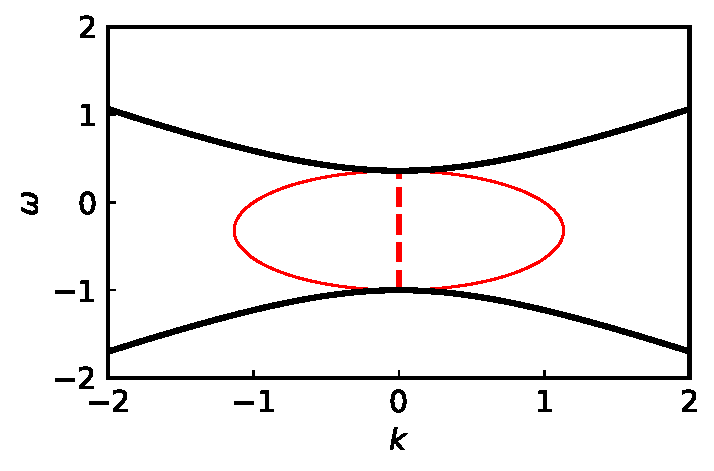
\includegraphics[width=\linewidth]{chapters/assets/dr/spectDBWC1DRDBMZAPltBlob}
\endminipage\hfill
\minipage{0.49\textwidth}
  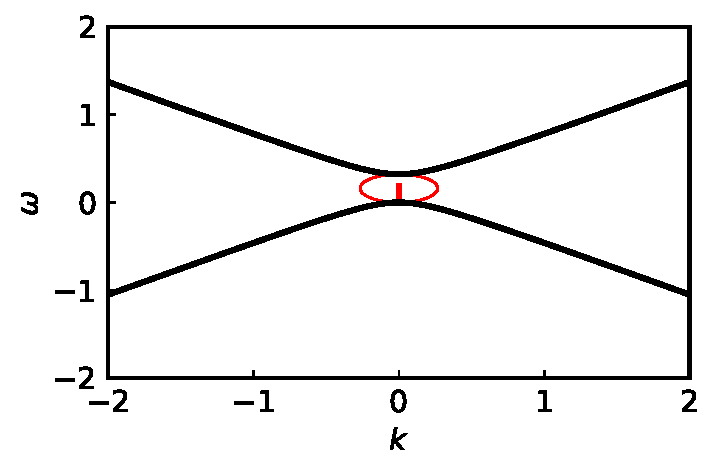
\includegraphics[width=\linewidth]{chapters/assets/dr/spectDBWC1DRDBMAAPltBlob}
\endminipage\hfill
\caption{The SS (left) and AS (right) of the dispersion relations for the two-angle model. The thick black curves represent $\omega(k)$ for real $k$. The red dashed and thin solid curves are $k_{\mathrm R}(\omega)$ and $k_{\mathrm R}(\omega) \pm k_{\mathrm I}(\omega)$ for real $\omega$ within the DR gap of $\omega$. Both $\omega$ and $k$ are measured in terms of the neutrino potential $\mu$.}
\label{fig-dr-db}
\end{figure}





% In core collapse supernova and neutron star mergers, neutrino emission is not in discrete zenith angles. Thus more realistic models involve continuous zenith angle ELN spectra. I reproduced the calculation in reference \cite{Izaguirre2016a} using the same Garching core-collapse supernova data set.\footnote{The data is from the Garching Core-Collapse Supernova Archive at \url{http://wwwmpa.mpa-garching.mpg.de/ccsnarchive/archive.html} } The spectrum shown in the left panel of Fig. \ref{fig-garching} is polynomial fitting of the Garching 1D supernova simulation data. On the right of Fig. \ref{fig-garching}, the dispersion relation for AS is shown as red (green, blue) solid lines. The instabilities associated with AS is shown as light red (light green, light blue) blobs. The two branches of SS solutions appear at the top half (AS+) and lower half (AS-). The result shows that instabilities occur either in region $\omega>0$ or region $\omega<0$ and with limits set the dispersion relation. I will prove that the instabilities appear between the dispersion relations and the axis $\omega=0$.


%@misc{garching-ccsn-data,
%mendeley-groups = {Neutrino/supernova},
%title = {{The Garching Core-Collapse Supernova Archive, http://wwwmpa.mpa-garching.mpg.de/ccsnarchive/archive.html}},
%url = {http://wwwmpa.mpa-garching.mpg.de/ccsnarchive/archive.html}
%}


\begin{figure}
   \minipage{0.49\textwidth}
     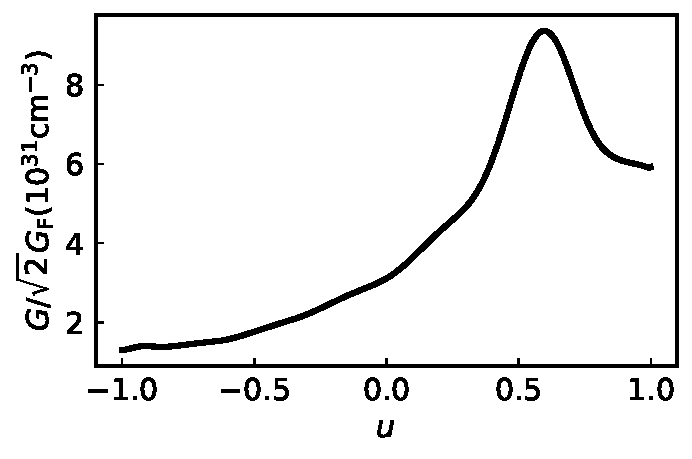
\includegraphics[width=\linewidth]{chapters/assets/dr/spectGarchingPlt.pdf}
   \endminipage\hfill
   \minipage{0.49\textwidth}
   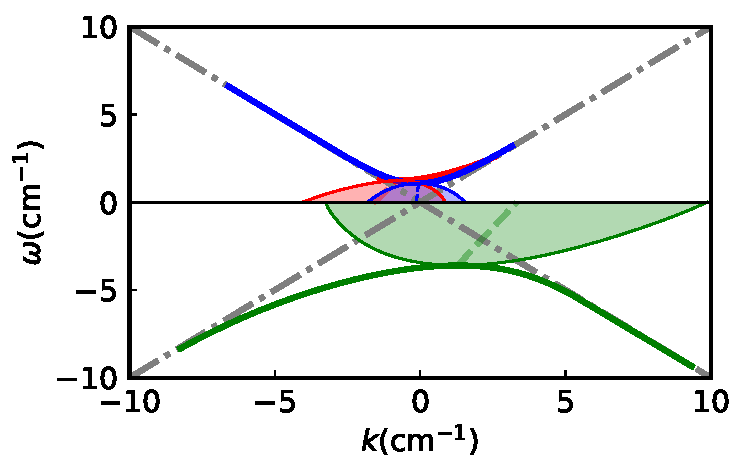
\includegraphics[width=\linewidth]{chapters/assets/dr/spectGarchingDRLSAPltBlob.pdf}
   \endminipage\hfill
   \caption{The SS$+$ (green), SS$-$ (blue) and AS (red) of the dispersion relations (right panel) for a net electron flavor neutrino density distribution $n_{\nu_{\ee}}(u) -n_{\bar\nu_\ee}(u)$ obtained from a Garching 1D supernova simulation (left panel). The thick solid curves represent the dispersion relations when both $\omega$ and $k$ are real. The dashed curves represent $k_{\mathrm R}(\omega)$ in the DR gap of $\omega$, and the thin solid curves (bounding the shaded regions) are $k_{\mathrm R}(\omega)\pm k_{\mathrm I}(\omega)$.}
   \label{fig-garching}
\end{figure}









\subsection{\label{chap:collective-sec:fast-mode-subsec:instability-to-gap}Refutation of the Conjecture}

The association of the flavor instability in space, i.e., $k_{\mathrm I}(\omega)\neq 0$, with a DR gap in $\omega$ seems fortuitous for the two-angle model. As I explained previously, for the two-angle model, the characteristic equations are quadratic equation of $k$ for any given $\omega$. Therefore there always exists a pair of complex solutions between the DR gap in $\omega$. This is not the case when the neutrinos are emitted with more than two zenith angles.

In Fig.~\ref{fig-dr-db-3}, I show the dispersion relations of a three-angle model with ELN
\begin{align}
    G(u) = 0.5\mu \delta(u+0.1) + \mu \delta(u - 0.4) + \mu \delta(u-0.6).
\end{align}
For this model, there exist complex solutions of $k(\omega)$ even though there is no DR gap in $\omega$. This is because the characteristic equations are cubic equations of $k$ for given $\omega$ which admit three solutions. In certain ranges of $\omega$ there is only one real solution of $k(\omega)$. The other two solutions must be complex which indicates flavor instabilities in space.


% Even though the DR gap of the  to instabilities works well for the models in \ref{chap:collective-sec:fast-mode-subsec:instabilities-and-gaps}, it can not be generalized to arbitrary number of emission angles nor to continuous spectra with crossings. As an example, I perform linear stability analysis of the three zenith angles emission configuration which is determined by a cubic function both in $\omega$ and $k$. Three solutions of $k(\omega)$ for given real $\omega(k)$  are expected. As long as real solutions disappear, complex solutions emerge, which leads to instabilities occur even without an actual gap. Rather the decrease in the number of real solutions for fixed $\omega$ or $k$ corresponds to the instabilities. As an example, I plotted in the lower panels of Fig.~\ref{fig-dr-db} the dispersion relations and instabilities for three zenith angles
% \begin{align}
%     G(u) = 0.5\mu \delta(u+0.1) + \mu \delta(u - 0.4) + \mu \delta(u-0.6)
%     % G(u) &= -0.5 \mu  \delta(u+0.1) + \mu \delta(u - 0.4) + \mu \delta(u-0.6) .
% \end{align}
% spectDBWC4 = {{0.5, -0.1}, {1, 0.4}, {1, 0.6}}
% spectDBC4 = {{-0.5, 0.1}, {1, 0.4}, {1, 0.6}}

% I also choose $\mu=1$ for the numerical calculations.
% For a given value of $\omega$ such as $\omega= 0.5$, the three AS solutions (Fig. \ref{fig-dr-db} lower left panel) of $k$ are $k=-4.6, 0.29, 1.2$. All three solutions are all real and indicate no spatial instabilities which is confirmed by calculation of instabilities shown as red blob. However, for another real $\omega = 0.2$, I find only one real solution $k=0.4$ from dispersion relation. The other solutions are complex and proven to be $k = -0.557106\pm 0.966535\mathrm i$ where the value with positive imaginary part leads to exponential growth. I conclude that instabilities doesn't require gap in dispersion relation except for two emission angles.

\begin{figure}[!htb]
    \minipage{0.49\textwidth}
      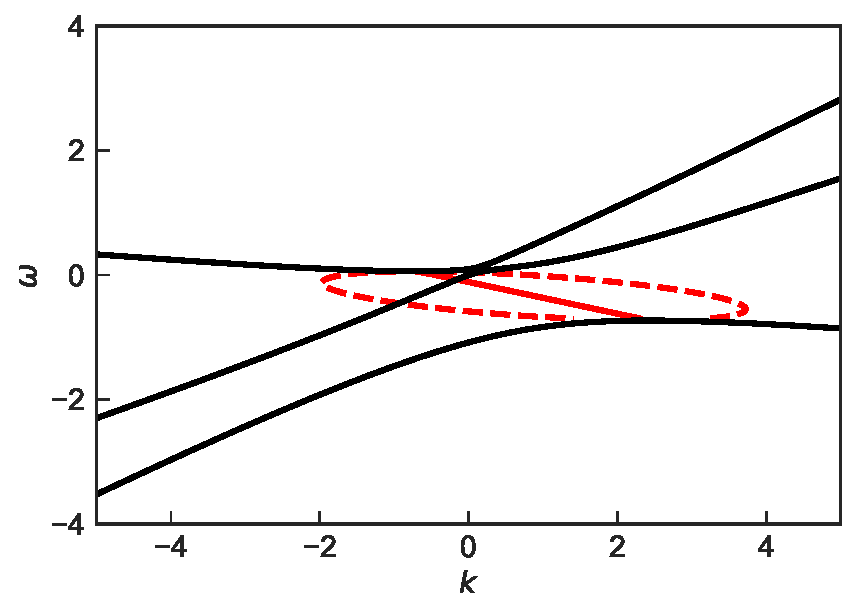
\includegraphics[width=\linewidth]{chapters/assets/dr/spectDB3WC4DRDBMZAPltBlob}
    \endminipage\hfill
    \minipage{0.49\textwidth}
      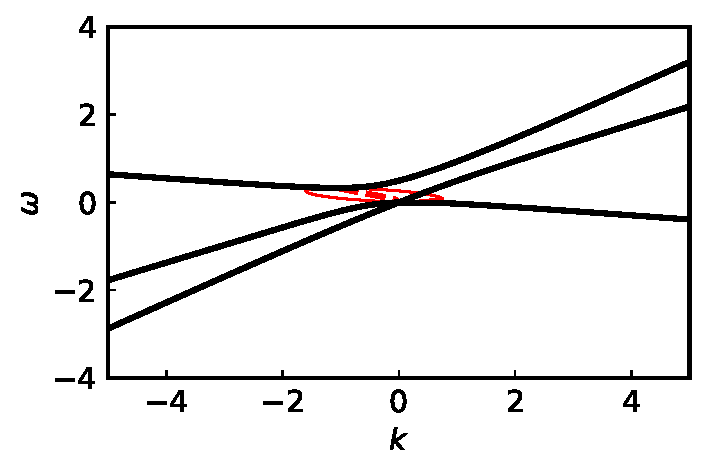
\includegraphics[width=\linewidth]{chapters/assets/dr/spectDB3WC4DRDBMAAPltBlob}
    \endminipage\hfill
    \caption{The same as Fig.~\ref{fig-dr-db} but for the three-angle model described in the text.}
    \label{fig-dr-db-3}
\end{figure}


The conjecture between the flavor instabilities and DR gaps does not work for the models with continuous ELN distribution $G(u)$ either. In Fig.~\ref{fig-box-c1} I show the dispersion relations for a step-like distribution
\begin{equation}
G(u) = \begin{cases}
-0.1 &  \text{if } -1 < u < -0.3, \\
1 &  \text{otherwise.}
\end{cases}
\label{chap:collective-sec:gap-eqn:eln-step-like}
\end{equation}
One sees that, for this model, the SS$+$ and SS$-$ solutions merge into a continuous DR curve so that there is no gap in $\omega$. However, there do exist complex solutions $k(\omega)$ for certain values of $\omega$.


% The instabilities for continuous emission angles do not necessarily correspond to the gap in dispersion relations either. In the earlier works of fast modes, Sawyer analyzed a box shaped angular distribution of neutrino emission \cite{Sawyer2016}. To address the generality of our conclusion, I repeat the calculation for box spectrum with crossing.
%
% I construct a box spectrum with value $-0.1$ within $u\in [-1,-0.3)$ and value $1$ within $u\in [-0.3,1]$ as shown in Fig.~\ref{chap:collective-sec:gaps-fig:box-spectrum}. As in the discrete emission case, I normalize all quantities using the maximum value of the spectrum. With the spectrum defined, I calculate the dispersion relation and find out complex values of $k$ for real $\omega$. The result shows that the dispersion relation of both AS solution and SS solution contains only one curve. No gap is formed but I observe instabilities between this curve and $\omega=0$ in AS solution as well as two unstable regions of $k$ in SS solution, which are plotted as red lines.


% \begin{figure}
%     \centering
%     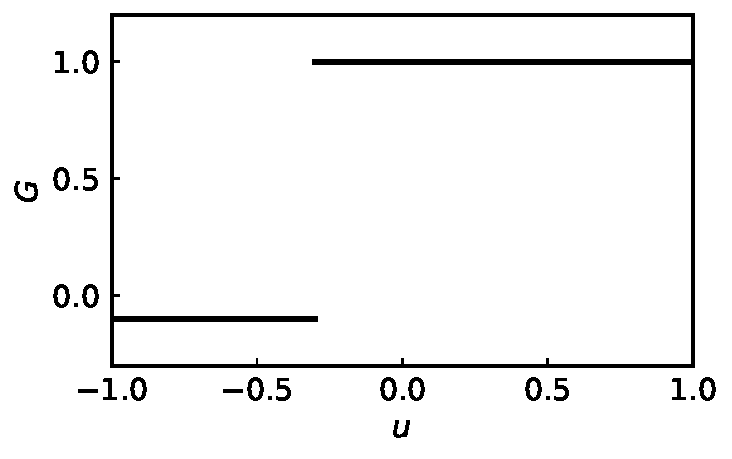
\includegraphics[width=0.5\textwidth]{chapters/assets/dr/boxSpectPlt}
%     \caption{
%     The box spectrum. I have used $G=-0.1$ for $u\in [-1,-0.3]$ and $G=1$ for $u\in [-0.3,1]$.
%     }
%     \label{chap:collective-sec:gaps-fig:box-spectrum}
% \end{figure}

\begin{figure}
   % \minipage{0.49\textwidth}
   %   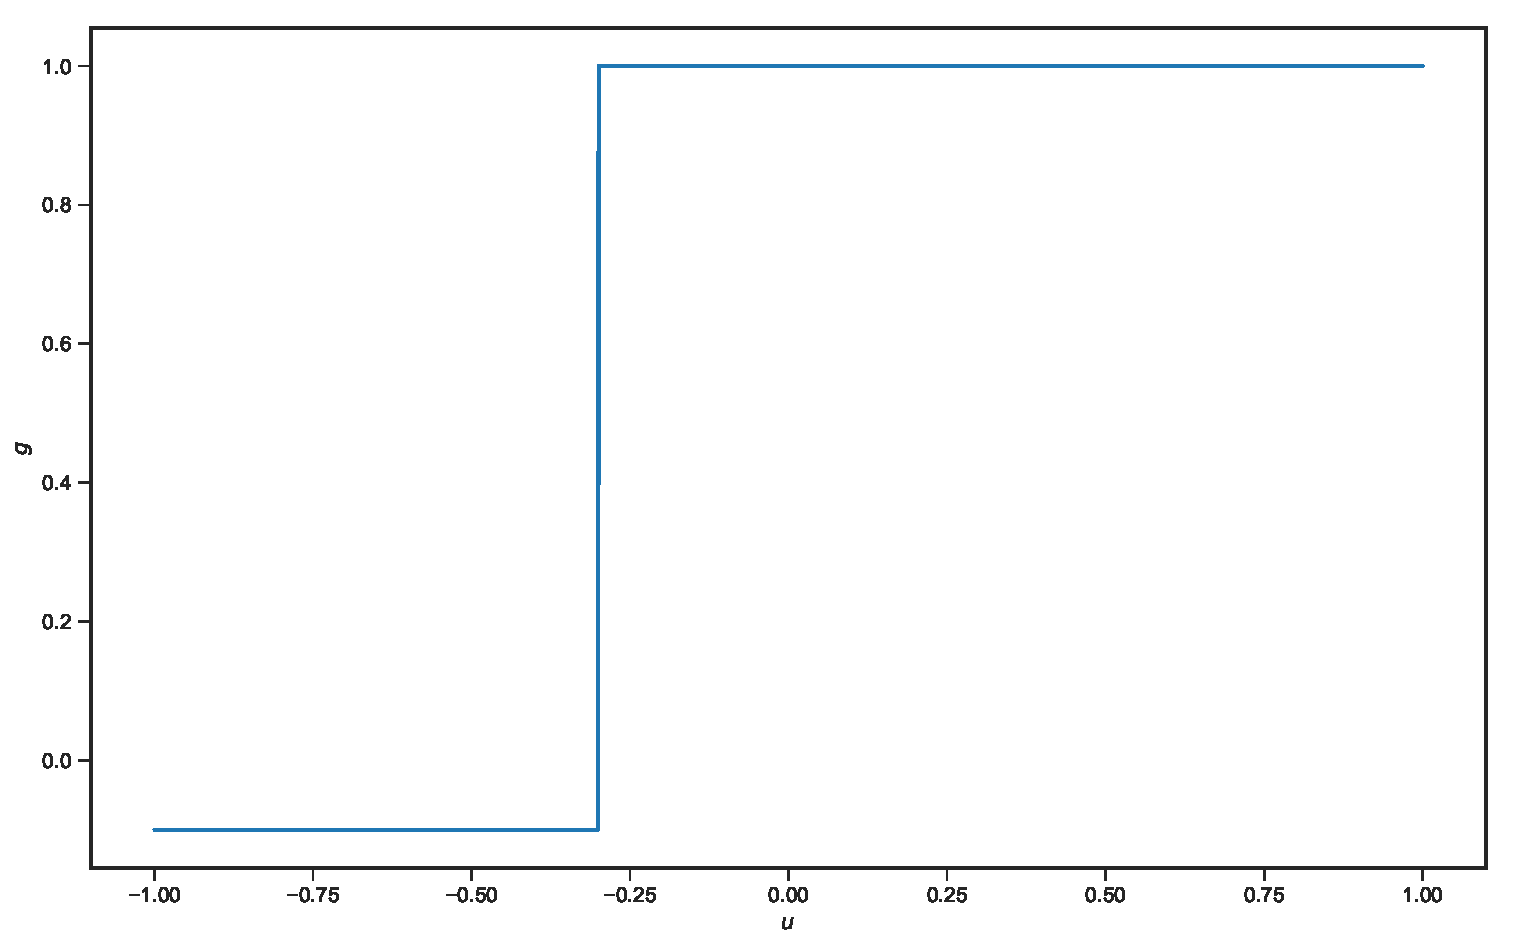
\includegraphics[width=\linewidth]{chapters/assets/dr/spectBoxC1Spectrum.pdf}
   % \endminipage\hfill
   \minipage{0.49\textwidth}
   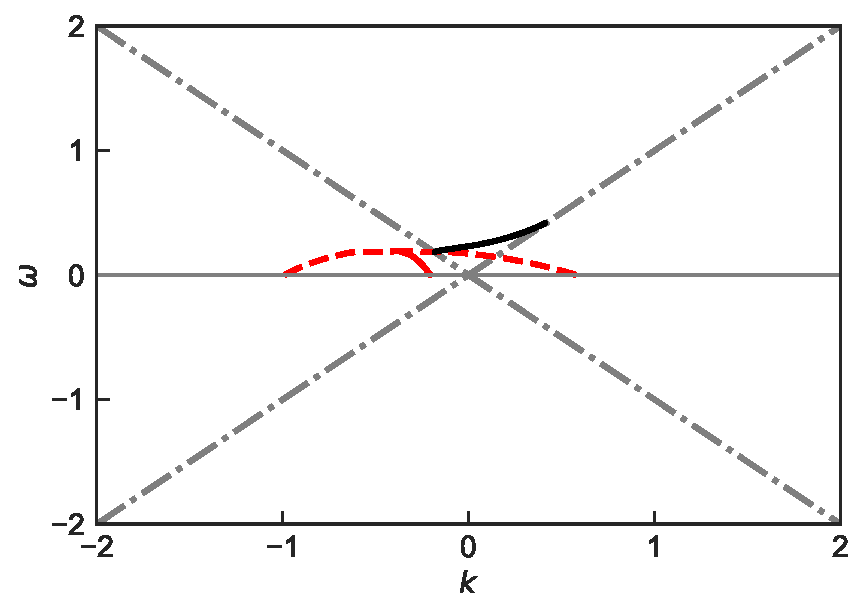
\includegraphics[width=\linewidth]{chapters/assets/dr/spectBoxC1MAADRPltBlob.pdf}
   \endminipage\hfill
   \minipage{0.49\textwidth}
   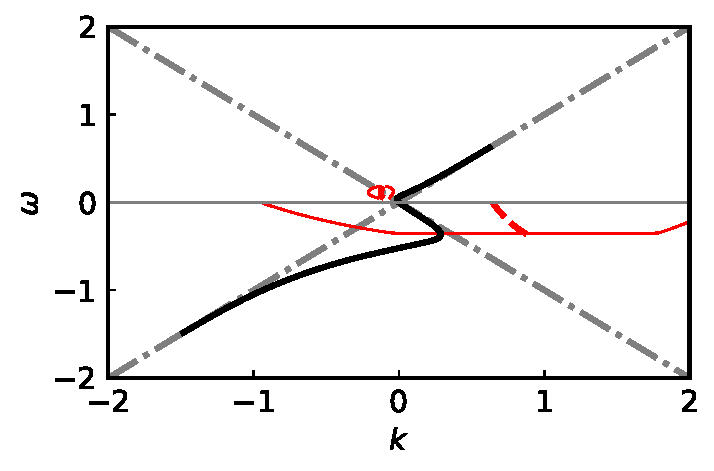
\includegraphics[width=\linewidth]{chapters/assets/dr/spectBoxC1MZADRPltBlob.pdf}
   \endminipage\hfill
   \caption{The same as Fig.~\ref{fig-dr-db} but for the ELN distribution in Eqn.~\eqref{chap:collective-sec:gap-eqn:eln-step-like}.
    }
   \label{fig-box-c1}
\end{figure}


%%%%%%%%%%%%%%%%%
%%

As shown in Fig.~\ref{fig-garching} and Fig.~\ref{fig-box-c1}, AS dispersion relations $k(\omega)$ appear only in the region where $\omega > 0$. This can be proved analytically as follows.
Suppose there exist dispersion relations $k(\omega) = k_{\mathrm R}(\omega) + k_{\mathrm I}(\omega)$ for $\omega \to 0$. Using Sokhotski–Plemelj theorem, I can rewrite the characteristic equation
\begin{equation}
   k = \frac{1}{4} \int \mathrm du G(u) \frac{ 1 - u^2 }{ \omega/k - u }.
   \label{chap:collective-eqn:k-omega-relation}
\end{equation}
as
\begin{subequations}
\begin{align}
k_{\mathrm R} =& \frac{1}{4}\left(  \mathcal{P} \int \mathrm d u G(u) \frac{ 1 - u^2 }{ - u }  \right)\label{eqn-re-k-arbitrary-spectrum} \\
k_{\mathrm I} =&  \frac{\pi}{4}G(0) \operatorname{Sign}\left( \omega \right) \operatorname{Sign}\left(  k_{\mathrm I}  \right),
\label{eqn-im-k-arbitrary-spectrum}
\end{align}
\label{eqn-k-arbitrary-spectrum}
\end{subequations}
where $\mathcal P$ denotes the principal value of the integral. As long as $G(0)\neq 0$, $\omega$ must have the same sign as $G(0)$ which implies that $k(\omega)$ exists only on one side of the vicinity of $\omega=0$. For the two scenarios depicted in Fig.~\ref{fig-garching} and Fig.~\ref{fig-box-c1}, $G(0)>0$ and $k(\omega)$ exist only in the upper half plane of $\omega$. This shows that, at least near $\omega =0$, the absence of a DR $\omega(k)$, i.e., a ``gap'' in $\omega$, is not always associated with the flavor instabilities in space.

Eqn.~\eqref{eqn-k-arbitrary-spectrum} can be used to determine the values of $k_{\mathrm R}$ and $k_{\mathrm I}$ in the limit of $\omega\to 0$ for the AS branch of the dispersion relations. One can apply the same method to the SS branches which gives
\begin{align}
&\left(4 k_{\mathrm R} - J_{-1} + J_1 \right)^2  - \left( \operatorname{Sign}(\omega k_{\mathrm I} )\pi G(0) +4 k_{\mathrm I} \right)^2 \nonumber\\
=& - \left( J_{-1} + J_1 \right) \pi \operatorname{Sign}(\omega k_{\mathrm I} ) G(0)
\label{chap:collective-eqn:dr-ss-general-limit-omega-0}
\end{align}
and
\begin{equation}
   k_{\mathrm I} = - \frac{\pi}{4} G(0) \operatorname{Sign}(\omega k_{\mathrm I} ) \left(  1 \pm \frac{ J_{-1} +  J_1 }{ 4 k_{\mathrm R} - J_{-1} + J_1}  \right),
   \label{chap:collective-eqn:dr-ss-general-limit-omega-0-ya}
\end{equation}
where
\begin{equation}
J_{n} = \mathcal P \int G(u)u^n \mathrm du,
\end{equation}
and the $+$ and $-$ signs are for SS$+$ and SS$-$, respectively. Eqn.~\eqref{chap:collective-eqn:dr-ss-general-limit-omega-0} and Eqn.~\eqref{chap:collective-eqn:dr-ss-general-limit-omega-0-ya} show that $k(\omega)$ exists on both sides of the vicinity of $\omega=0$ but may be different for SS$+$ and SS$-$.


% In the case that the smooth and continuous ELN spectrum doesn't go through $0$ values (no crossing), the gap in dispersion relations indeed indicates instabilities, as shown in reference \cite{Izaguirre2016a}. I can prove that the instabilities in non-AS, AS+, or AS- solution can only appear in either region $\omega\leq 0$ or region $\omega \geq 0$. As it suggests, the instability regions propagate only between the dispersion relation curves and the axis $\omega=0$. Suppose I am looking for complex solutions for given real omega as in Fig. \ref{fig-garching}, AS solution Eq. \eqref{eqn-maa} is rewritten as a function $k(\omega/k)$. More explicitly, I have to solve the integral function to find out $k$ for real $\omega$,
% \begin{equation}
%    k = \frac{1}{4} \int \mathrm du G(u) \frac{ 1 - u^2 }{ \omega/k - u }.
%    \label{eqn-k-omega-relation}
% \end{equation}
% To investigate how instabilities developed around the horizontal  axis, I solve Eq. \eqref{eqn-k-omega-relation} in the limit $\omega\to 0$. For complex $k$, the integral can be decomposed into the principal value $\operatorname{Re}(k)$ and imaginary part $\operatorname{Im}(k)$ using Sokhotski–Plemelj theorem,
% \begin{subequations}
% \begin{align}
% \operatorname{Re}(k) =& \frac{1}{4}\left(  \mathcal{P} \int \mathrm d u G(u) \frac{ 1 - u^2 }{ - u }  \right)\label{eqn-re-k-arbitrary-spectrum} \\
% \operatorname{Im}(k) =&  \frac{\pi}{4}G(0) \operatorname{Sign}\left( \omega \right) \operatorname{Sign}\left(  \operatorname{Im}(k)  \right).
% \label{eqn-im-k-arbitrary-spectrum}
% \end{align}
% \end{subequations}
% Assuming no crossing is found in spectrum $G(u)$ at $u=0$, Eq. \eqref{eqn-im-k-arbitrary-spectrum} shows that $\omega$ must have the same sign as $G(0)$ if I find nonzero imaginary part in $k$. I conclude that instabilities can only grow either in the upper plane $\omega>0$ or lower plane $\omega<0$. What's more, the value of $k$ at limit $\omega\to 0$ can be solved out of Eq. \eqref{eqn-re-k-arbitrary-spectrum} and Eq. \eqref{eqn-im-k-arbitrary-spectrum}. For instabilities the imaginary part of $k$ tells us the growth rate is,
% \begin{equation}
%    \lvert \operatorname{Im}(k) \rvert  =  \frac{\pi}{4}\lvert G(0)\rvert .
% \end{equation}
% Similar result is obtained for SS solutions,
% \begin{align}
% &\left(4\operatorname{Re}(k) - \mathcal P \int \frac{G(u)}{u} \mathrm d u + U_1 \right)^2  - \left( \operatorname{Sign}(\omega \operatorname{Im}(k) )\pi G(0) +4 \operatorname{Im}(k) \right)^2 \\
% =& - \left( \mathcal P \int \frac{G(u)}{u} \mathrm du + U_1 \right) \pi \operatorname{Sign}(\omega \operatorname{Im}(k) ) G(0),
% \end{align}
% where $U_m = \int G(u) u^m \mathrm du$ and all the integrals are over all the spectrum. The equations are quadratic in both $\operatorname{Re}(k)$ and $\operatorname{Im}(k)$ so the real solutions can be calculated and verified with linear stability analysis. The imaginary part $\operatorname{Im}(k)$
% \begin{equation}
%    \operatorname{Im}(k) = - \frac{1}{4} \pi G(0) \operatorname{Sign}(\omega \operatorname{Im}(k) ) \left(  1 \pm \frac{ \mathscr P \int \frac{G(u)}{u} du + \int G(u) u du }{ 4 \operatorname{Re}(k) - \mathscr P \int \frac{G(u)}{u} du + \int G(u) u du }  \right)
% \end{equation}
% determines that the two different solutions are either in the region $\omega>0$ or in the region $\omega<0$ which corresponds to SS$+$ and SS$-$ solutions. The instabilities in the two regions are not continuous at $\omega=0$.






%%%%%%%%%%%%%%%%%%%%%%%%%%%%%%%%%%%%%%%%%%%%%%%%%%%%%%%%%%%%%%%%%%%%%%%%%
%%%%%%%%%%%%%%%%%%%%%% Neutrino Halo Problem %%%%%%%%%%%%%%%%%%%%%%%%%%%%
%%%%%%%%%%%%%%%%%%%%%%%%%%%%%%%%%%%%%%%%%%%%%%%%%%%%%%%%%%%%%%%%%%%%%%%%%





\section{\label{chap:halo}Neutrino Oscillations with Reflected Fluxes}

Most of the researches on supernova neutrino oscillations assumed that neutrinos are emitted from the spherical surface of a neutron star and that they are free streaming. In the real supernova environment, however, a small amount of neutrinos can be scattered back towards the neutron star. J. Cherry et al. showed that the ``neutrino halo'' formed by the scattered neutrino fluxes can change the neutrino self-interaction potential dramatically  which may have an impact on neutrino oscillations in the supernova~\cite{Cherry2012}. In the section, I describe a toy model which can be used to explore the impact of the scattered neutrino fluxes on neutrino oscillations.

% One of the big questions about neutrino oscillations in supernovae is the so called halo problem.
% J. Cherry et al showed that neutrino flavor conversions are greatly affected by the back scattered neutrinos in supernovae, which is called the neutrino halo problem~\cite{Cherry2012}. Neutrinos around supernovae are scattered and some of them are scattered to move almost backward. On the other hand, neutrino self-interactions is proportional to the inner product of momenta of neutrinos, which leads to the dependence on $1-\cos\theta$ where $\theta$ is the angles between momenta of two neutrinos. Most of the research has been concentrating on mostly forward scattering, with small values for $1-\cos\theta$. For backward scattered neutrinos, the interaction potential can be much larger than the forward scattered neutrino potential. Though the work by S. Sarikas et al showed that matter suppression is still significant within this region~\cite{Sarikas2012a}, it is not clear how exactly the neutrino halo alters neutrino oscillations. The halo problem itself is worth more calculations. In this chapter, I will present a relaxation method for this problem. The focus will be on the numerical method itself.


\subsection{Two-Beam Model with Reflection}

I will consider the two-beam model depicted in Fig.~\ref{chap:collective-sec:two-beams-fig:two-beam-line-model} but with a ``neutrino mirror'' at $z=L$ that partially reflects the neutrino beams backward without changing their flavor content. The equations of motion for neutrino oscillations in this model are
\begin{align}
    \ri \sin\theta_1 \partial_z \rho_1 = & [ \mathsf H_1, \rho_1 ], \\
    \ri \sin\theta_2 \partial_z \rho_2 = & [ \mathsf H_2, \rho_2 ], \\
    -\ri \sin\theta_3  \partial_z \rho_3 = & [ \mathsf H_3, \rho_3 ], \\
    -\ri \sin\theta_4 \partial_z \rho_4 = & [ \mathsf H_4, \rho_4 ],
\end{align}
where beams 1 and 2 contain neutrinos and antineutrinos, beams 3 and 4 are the reflected fluxes of 1 and 2, respectively, with $\theta_3=\theta_1$ and $\theta_4=\theta_2$. The Hamiltonians in the vacuum mass basis are
\begin{align}
    \mathsf H_1 =& -\eta \omega_\vv \sigma_3 + \mu( -\alpha \chi_-  \rho_2 - \alpha \chi_+ R \rho_4 + \chi_1 R  \rho_3), \\
    \mathsf H_2 =& \eta \omega_\vv \sigma_3 + \mu( \chi_- \rho_1 -\alpha \chi_2 R  \rho_4 + \chi_+ R  \rho_3), \\
    \mathsf H_3 =& -\eta \omega_\vv \sigma_3 + \mu( -\alpha R  \chi_-  \rho_4 -\alpha \chi_+ \rho_2 + \chi_1  \rho_1), \\
    \mathsf H_4 =& \eta \omega_\vv \sigma_3 + \mu( R   \chi_- \rho_3 + \chi_+  \rho_1 -\alpha \chi_2  \rho_2),
\end{align}
where $\mu=\sqrt{2}G_{\mathrm F}n_1$ with $n_1$ being the number flux of beam 1, $\alpha=n_2/n_1$, $R$ is the reflection coefficient of the ``neutrino mirror'', and
\begin{align*}
    \chi_+ = & 1 - \cos ( \theta_1 + \theta_2 ), \\
    \chi_- = & 1 - \cos ( \theta_1 - \theta_2 ), \\
    \chi_1 = & 1 - \cos ( 2\theta_1 ), \\
    \chi_2 = & 1 - \cos ( 2\theta_2 ).
\end{align*}




\subsection{\label{chap:halo-sec:num}Relaxation Method}



I developed a relaxation method to solve the two-beam model with reflection numerically. For the purpose of illustrating the algorithm, I denote the Hamiltonian using its components in flavor space:
\begin{equation}
\mathsf H = -\sum_i \frac{H_i}{2}\sigma_i.
\end{equation}
At position $z$, the evolution operator $\mathsf U(\Delta l,z)$ is
% \begin{equation}
%     \mathsf U(t+\Delta t, t) = \begin{pmatrix}
%         \cos\left( \frac{H \Delta t}{2} \right) + \ri \frac{H_3}{H} \sin \left( \frac{H \Delta t}{2} \right) &  \ri \frac{H_1 - \ri H_2}{H} \sin \left( \frac{H \Delta t}{2} \right)  \\
%         - \ri \frac{ H_1 -\ri H_2}{H} \sin \left( \frac{H \Delta t}{2} \right) & \cos\left( \frac{H \Delta t}{2} \right) - \ri \frac{H_3}{H} \sin \left( \frac{H \Delta t}{2} \right)
%     \end{pmatrix}
% \end{equation}
% is the length of the Hamiltonian in flavor space. The evolution operator can also be expanded using the Pauli matrices
\begin{align}
    U(\Delta l, z) = \cos \left( \frac{H \Delta l}{2} \right) \mathsf I + \ri \left( \frac{H_1}{H}  \sigma_1 + \frac{H_2}{H} \sigma_2 + \frac{H_3}{H} \sigma_3 \right) \sin \left( \frac{H \Delta l}{2} \right)
    % \cos \left( \frac{H \Delta t}{2} \right) \mathsf I + \ri \frac{H_1}{H} \sin \left( \frac{H \Delta t}{2} \right) \sigma_1 + \ri \frac{H_2}{H} \sin \left( \frac{H \Delta t}{2} \right) \sigma_2 + \ri \frac{H_3}{H} \sin \left( \frac{H \Delta t}{2} \right) \sigma_3
    % & \equiv -\frac{1}{2} \left( U_0 \mathsf I + U_1 \sigma_1 + U_2 \sigma_2 + U_3 \sigma_3 \right).
\end{align}
where $\Delta l$ is the propagation distance along the neutrino trajectory, and
\begin{equation}
    H = \sqrt{ H_1^2 + H_2^2 + H_3^2 }.
\end{equation}
Then I calculate the density matrix at the new position $z'$ as
\begin{align}
    \rho ( z' ) &= \mathscr F ( \mathsf H(z), \rho(z), \Delta l ) \\
     &= \mathsf U (\Delta l, z) \rho(t)U^\dagger (\Delta l, z) \\
    & = \frac{1}{4} \sum_j \left[  \cos( H \Delta l) \rho_j - \frac{2}{H^2} \sin^2 \left( \frac{H \Delta l}{2} \right)  \sum_i H_i \rho_i H_j  \right] \sigma_j.
\end{align}
I discretize the $z$ axis into $N$ bins with $\Delta z = L/N$ and $z_n=n \Delta z$ ($n=0,1,\cdots, N$). I use the evolution operator $U_a(z+\Delta z, z)$ and the following iteration algorithm until I achieve numerical convergence.
% \begin{algorithm}
%     \caption{Relation method for neutrino oscillations with reflections.}\label{alg:rela}
%     \begin{algorithmic}[1]
%     \Procedure{Euclid}{$a,b$}\Comment{The g.c.d. of a and b}
%     \State $r\gets a\bmod b$
%     \While{$r\not=0$}\Comment{We have the answer if r is 0}
%     \State $a\gets b$
%     \State $b\gets r$
%     \State $r\gets a\bmod b$
%     \EndWhile\label{euclidendwhile}
%     \State \textbf{return} $b$\Comment{The gcd is b}
%     \EndProcedure
%     \end{algorithmic}
% \end{algorithm}
% \begin{algorithm}[H]
%       \(\rho\)
%     % \KwData{The neutrino states at $z=0$}
%     \KwResult{Relax the neutrino oscillations to equilibrium}
%     Calculate the state of the forward beam using null backward beam\;
%     \While{ neutrino states not close enought to the previous step }{
%         calculate the backward beam and forward beam together using the state of beams from the previous iteration.
%     }
%     % \caption{Relation method for neutrino oscillations with reflections.}
% \end{algorithm}
\begin{lstlisting}[mathescape]
for all a, n: #a -> beam index; n -> position index
    $\rho^0_a$ ($z_n$) = 0
for all a:
    $\rho^0_a$ ($a_0$) = [ [ 1, $\epsilon_a$ ], [ $\epsilon_a^*$, 0 ] ]
j = 0 #j -> iteration index
do:
    for a = 1, 2 and n < N:
        $\rho_a^{j+1}$ ($z_{n+1}$) = $\mathscr{F}$( $H^{j}_a$ ($z_n$), $\rho_a^j$($z_n$), $\Delta z/\sin \theta_a$ )
    for a = 3, 4 and n > 0:
        $\rho_a^{j+1}$ ($z_{n-1}$) = $\mathscr{F}$( $-H^{j}_a$ ($z_n$), $\rho_a^j$($z_n$), $\Delta z/\sin \theta_a$ )
while $\vert \rho^{j+1} - rho^{j} \vert$ > error tolerance
\end{lstlisting}
To speed up the calculations, I have parallelized the above algorithm with OpenMP.



% \begin{enumerate}
%     \item
% Calculate the state of the forward beam using null backward beam;
% \item
% Calculate the backward beam and forward beam together using the state of beams from the previous step current counter beams;
% \item
% Repeat the previous step until the state of the beams reach equilibrium.
% \end{enumerate}

% In Fig.~\ref{chap:halo-sec:num-fig:compare-vac-bipolar-validate}, I plotted the neutrino oscillations for several different different reflection coefficients $R=0, 0.1, 0.2$. The forward beam for $R=0$ should be the same as vacuum oscillations which is shown in gray

% and bipolar models. The reason that we still have conversions is because of the vacuum term, which is additional to linear stability analysis (see Fig.~\ref{chap:halo-sec:num-fig:compare-vac-bipolar-lsa}).
%I also proved that the neutrino oscillations reached equilibrium quickly as shown in Fig.~\ref{chap:halo-sec:num-fig:relax-color} where the neutrino flavors are indicated by colors.






% \begin{figure}[htbp]
%     \minipage{\textwidth}
%     % 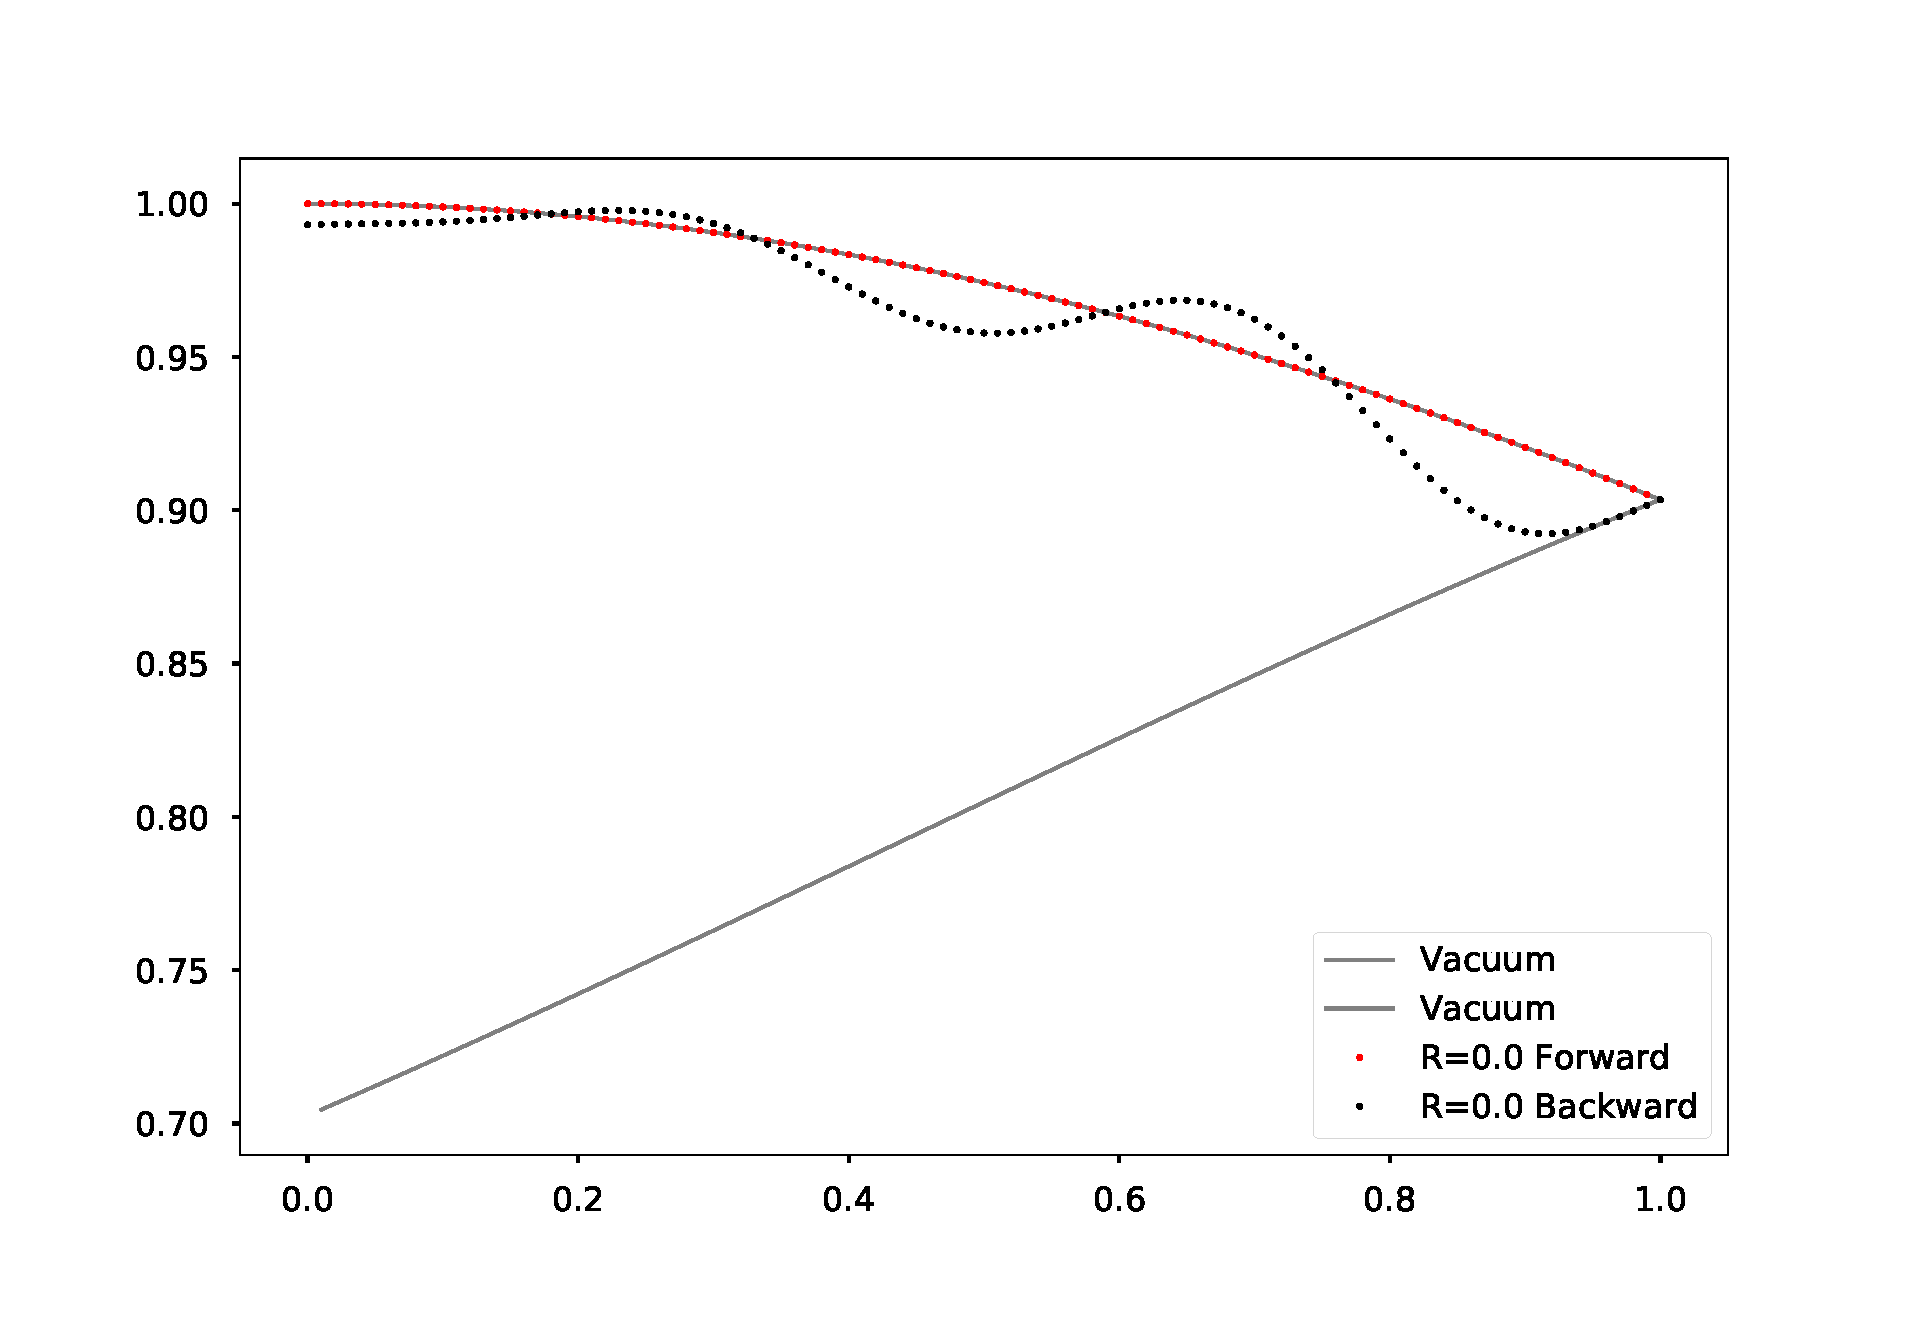
\includegraphics[width=\textwidth]{chapters/assets/halo/halo-mu-4-compare-vac.pdf}
%     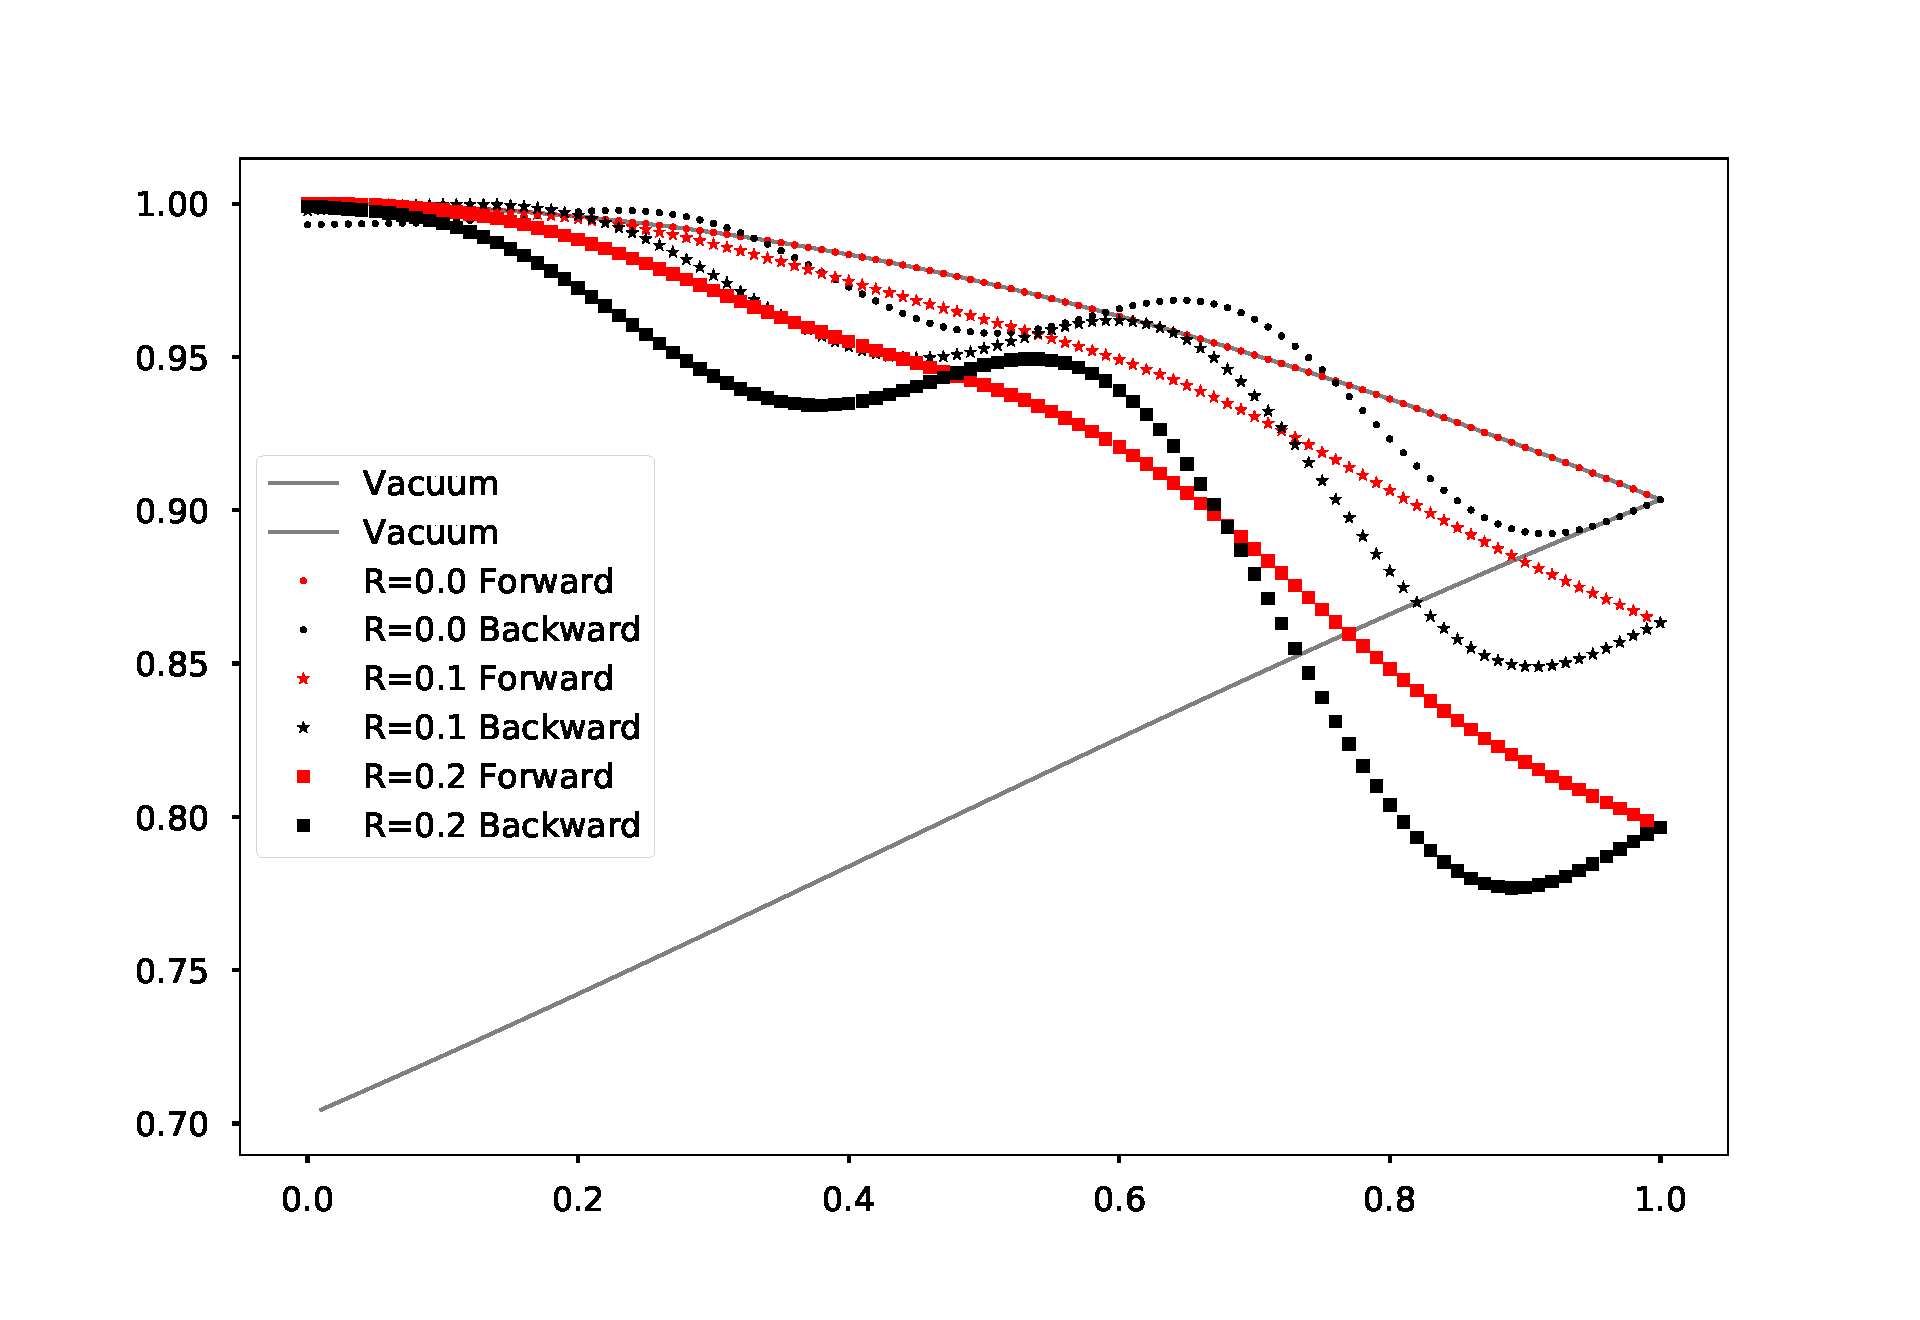
\includegraphics[width=0.49\textwidth]{chapters/assets/halo/halo-mu-4-r-multiple.pdf}
%     \endminipage\hfill
%     \minipage{\textwidth}
%     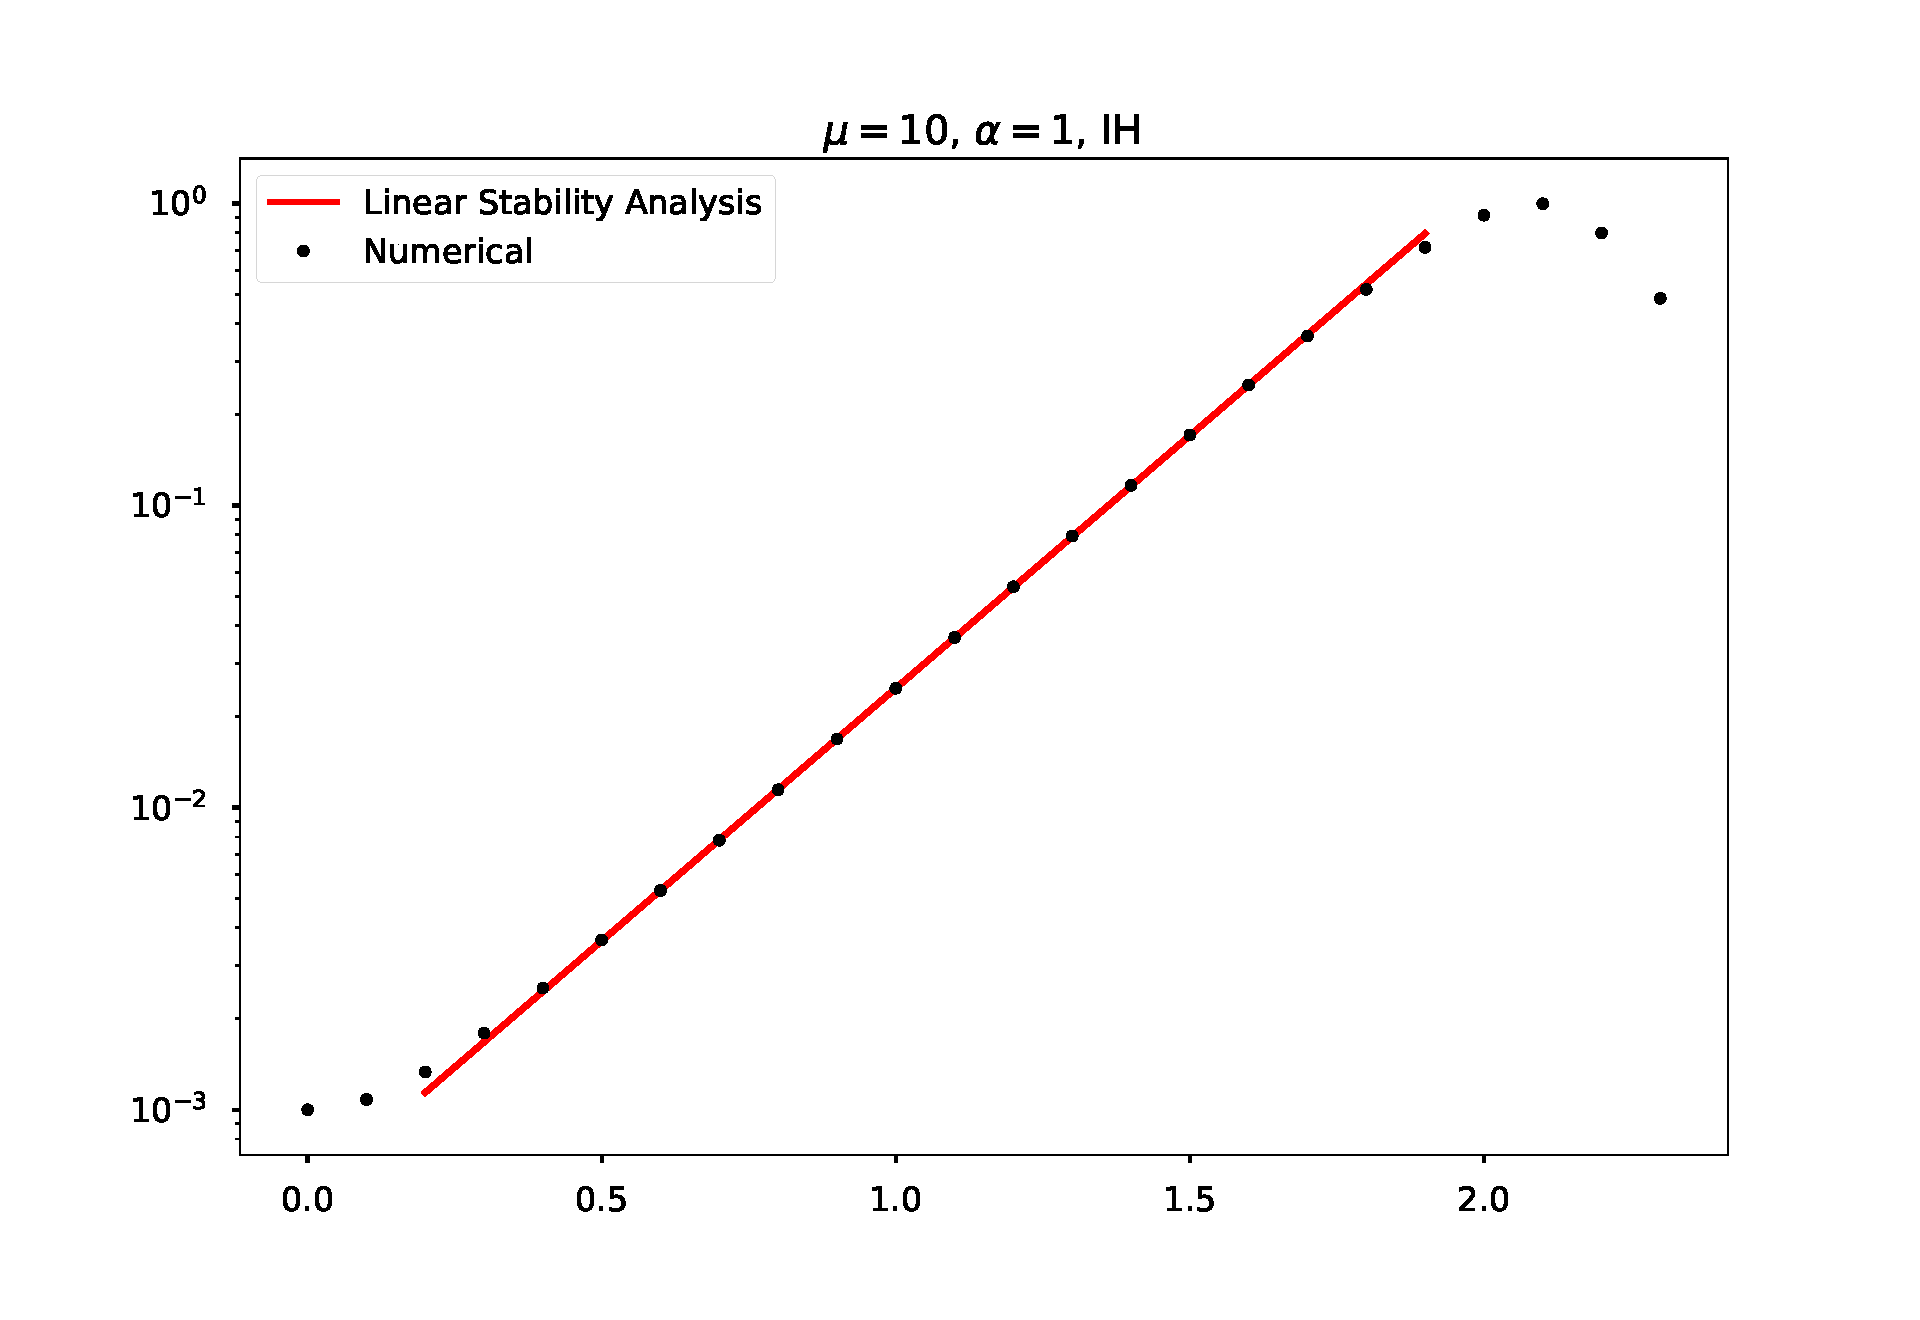
\includegraphics[width=0.49\textwidth]{chapters/assets/halo/halo-mu-4-compare-bipolar.pdf}
%     \endminipage\hfill
%     \caption{The left panel validates code by setting reflection to zero and approach vacuum for single forward beam. Meanwhile, we notice that for nonzero reflections, more conversion is done, which makes sense due to the similarity between $R$ and the asymmetry parameter $\alpha$ in bipolar model. The right panel validates the code by setting reflection to zero and compare with bipolar model for two beams case, where the slope is matching the theoretical value $3.85$.}
%     \label{chap:halo-sec:num-fig:compare-vac-bipolar}
% \end{figure}


%%%%%%%%%%%%%%%%%%%%%%%%%
%%% Equilibrium
% \begin{figure}[htbp]
%     \centering
%     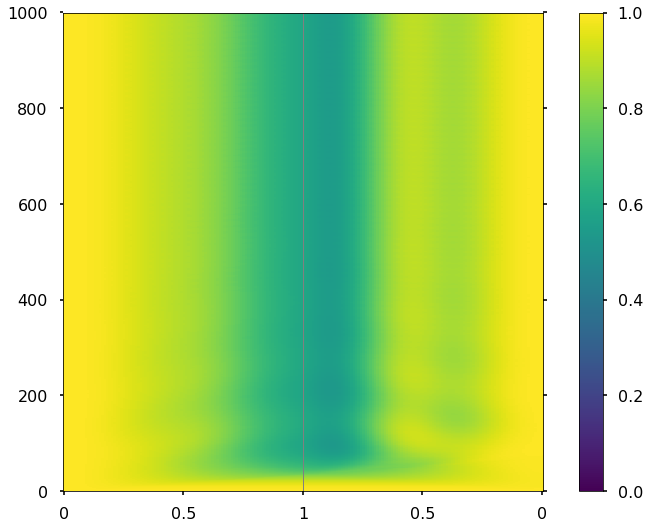
\includegraphics[width=0.8\textwidth]{chapters/assets/halo/relax-color.png}
%     \caption{Relaxation method reaches equilibrium after some steps. The horizontal axis is the $z$ direction while the vertical axis is the number of iteration steps. The color indicates the survival probability for electron flavor. This calculation sets $\mu = 4$, $R=0.2$, and is done within range $[0,1]$. Equilibrium is reached around step 400 and the neutrino states stays in equilibrium.}
%     \label{chap:halo-sec:num-fig:relax-color}
% \end{figure}




% \subsection{\label{chap:halo-sec:line}Line Model}

% I will use the line model to build intuitions of the halo problem. The halo problem is simplified to have neutrinos emitted from a line $z=0$ homogeneously, which are reflected from a certain distance $z=L$. In general, the reflection angles doesn’t have to be Snell’s law. The scattering can be in any angle with different amplitudes. Here I am using this very simple Snell’s law just to explore the effect of halo. In summary, I use the following assumptions.
% \begin{itemize}
%     \item Neutrinos are emitted from a line, which is not the case in a real supernova.
%     \item Neutrinos are emitted with translation symmetry on the line. Breaking the symmetry might bring in other qualitatively different results.
%     \item Neutrinos are reflected from a certain surface $z=L$, which is different from reality where neutrinos are scattered everywhere.
%     \item Neutrinos are reflected according to Snell's law.
%     \item Neutrinos are homogeneously reflected at $z=L$.
% \end{itemize}

% Fig.~\ref{chap:halo-sec:line-fig:line-model} describes the above model in details. The state of the left-going beam and right-going beam are denoted as $\rho_1$ and $\rho_2$, respectively. The forward beams have neutrino number densities $n_i$ while the reflected beams have neutrino number densities $R n_i$.

% \begin{figure}
%     \centering
%     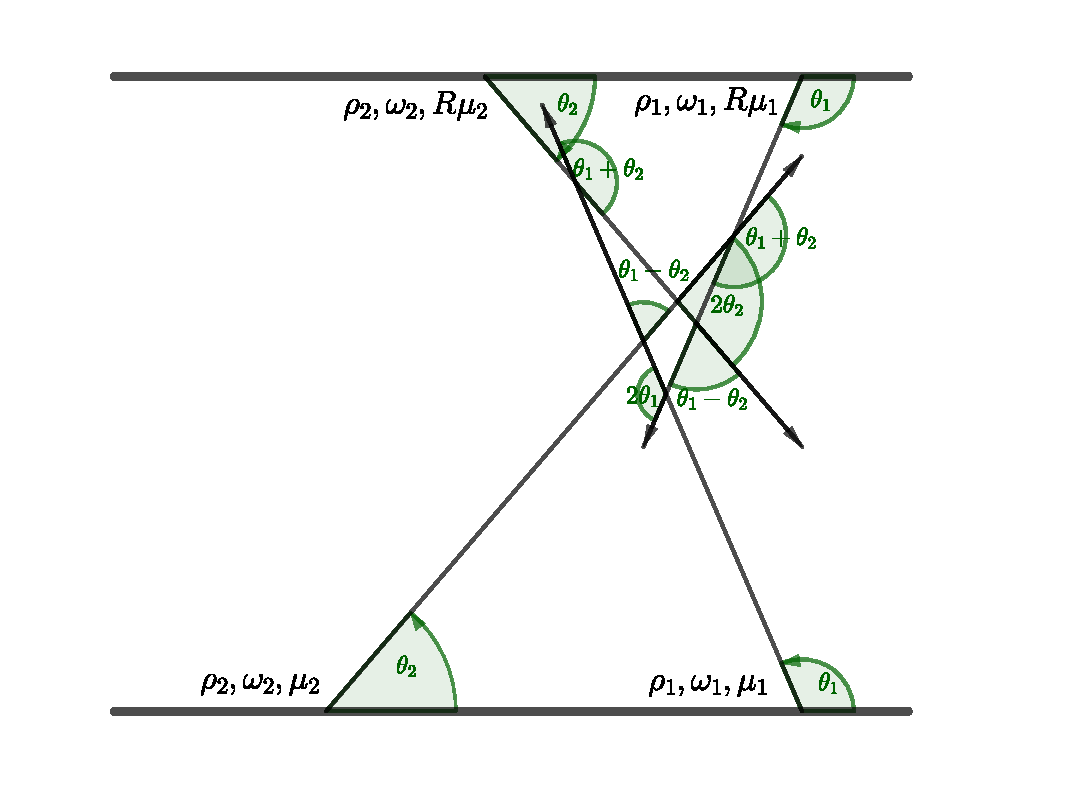
\includegraphics[width=\textwidth]{chapters/assets/halo/halo-line-model}
%     \caption{A general line model for the halo problem. The neutrinos are emitted from the bottom surface $z=0$ and reflected at the top surface $z=L$. Two neutrino beams are demonstrated in the figure.}
%     \label{chap:halo-sec:line-fig:line-model}
% \end{figure}




\subsection{\label{chap:halo-sec:line-sym}Validation of the Relaxation Method with Relected Single-Neutrino-Beam}


As a check to the relaxation algorithm discussed in the previous subsection, I apply it to the single-beam model with reflection, i.e., $\theta_1=\pi/2$ and $\alpha=0$. As the first step of the validation of the numerical code, I compare the numerical and analytical results for the vacuum oscillations case with $R=0$ and the normal neutrino mass hierarchy. The results are shown in Fig.~\ref{chap:halo-sec:num-fig:compare-vac-validate}.

\begin{figure}[htbp]
    \centering
    % 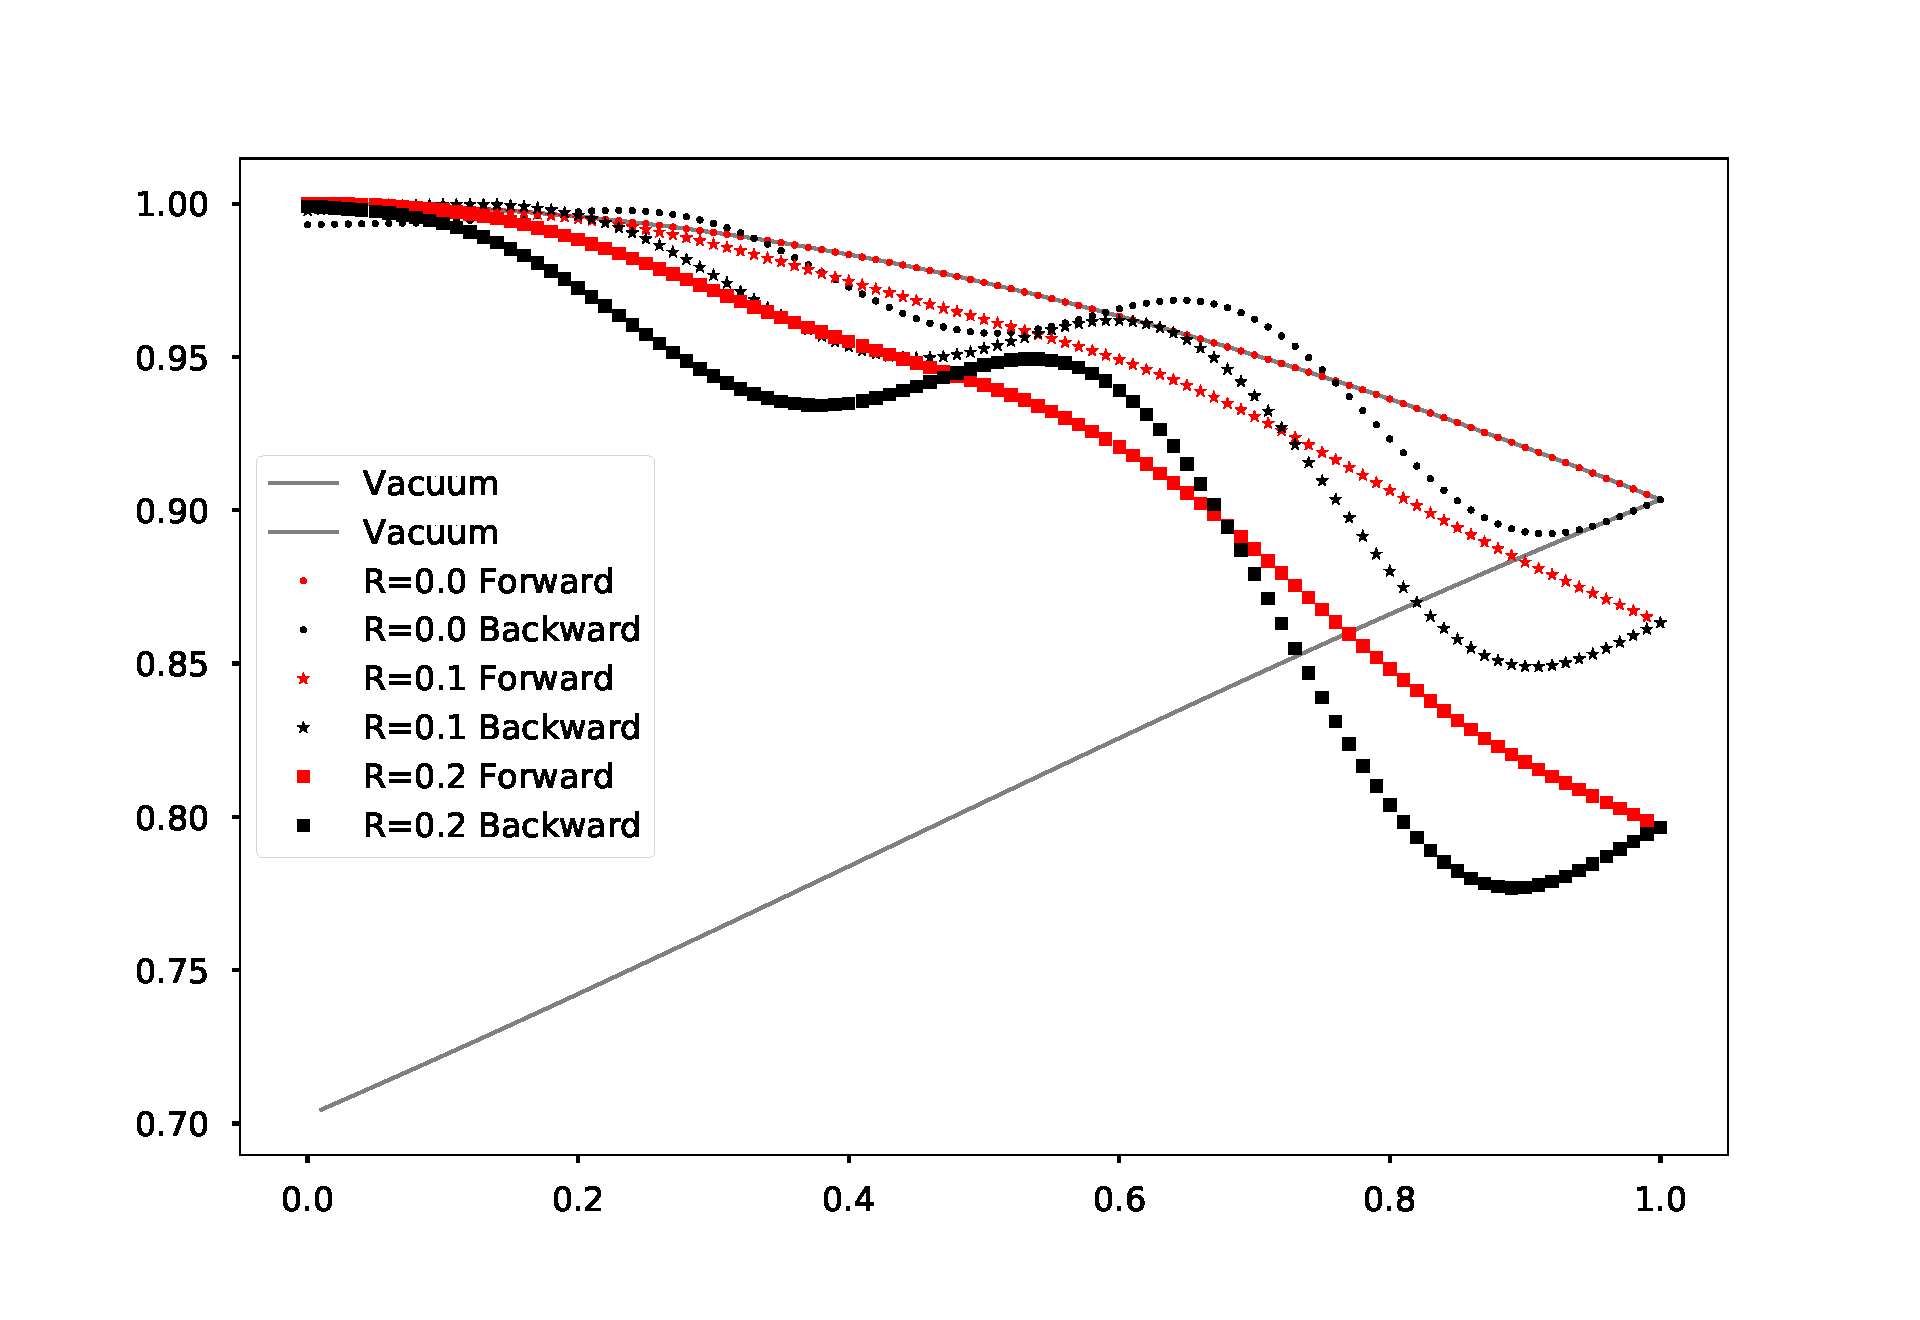
\includegraphics[width=\textwidth]{chapters/assets/halo/halo-mu-4-r-multiple.pdf}
    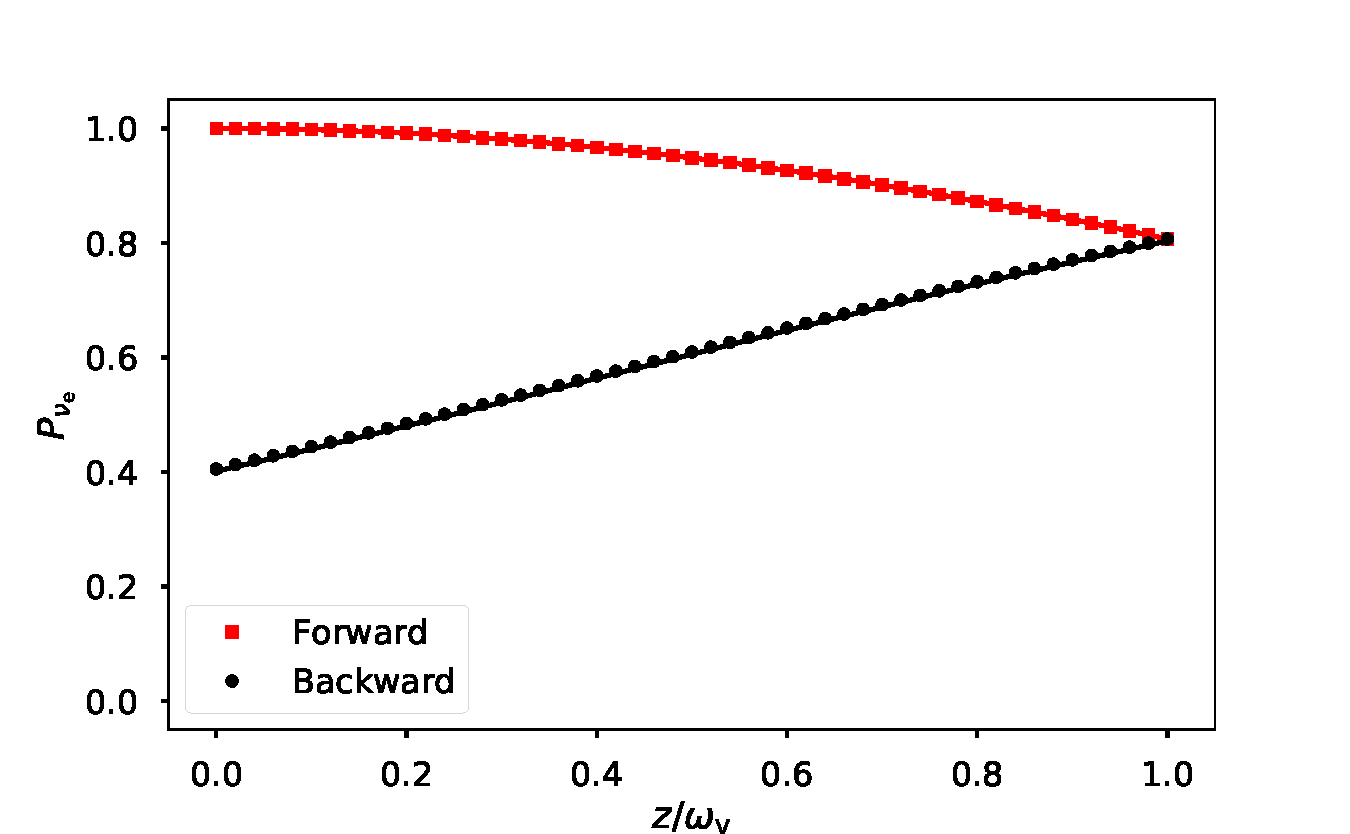
\includegraphics[width=\textwidth]{chapters/assets/halo/validate-using-vacuum-r-0-mu-1}
    \caption{The validation of the numerical code for the single-beam model with $R=0$ and $L=1/\omega_\vv$. The markers and the continuous curves represent the numerical and analytical results, respectively. }
    \label{chap:halo-sec:num-fig:compare-vac-validate}
\end{figure}
% \begin{figure}
%     \centering
%     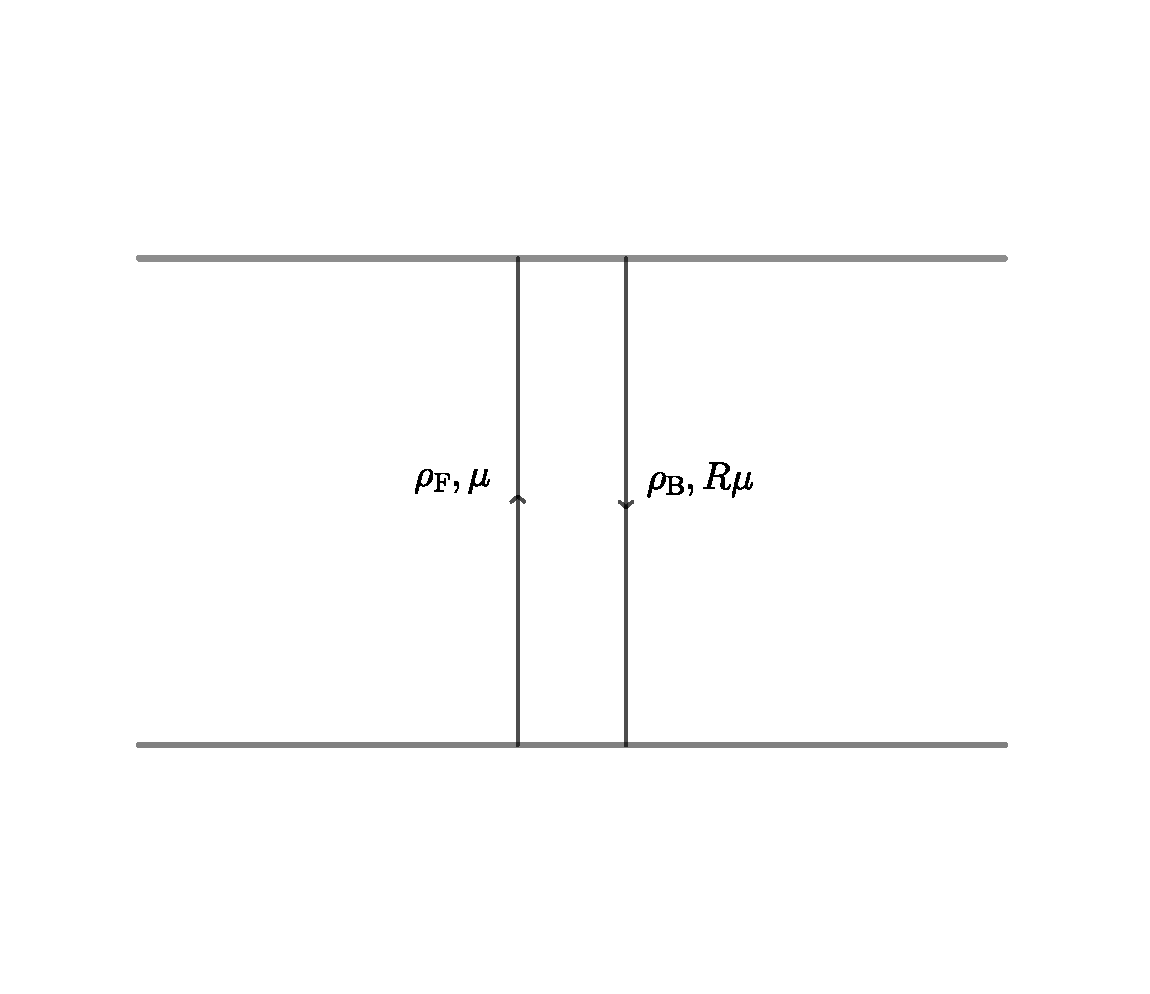
\includegraphics[width=\textwidth]{chapters/assets/halo/halo-line-model-single-beam}
%     \caption{The single-neutrino-beam line model with $\theta=\pi/2$. The neutrinos are emitted from $z=0$ and reflected at $z=L$.}
%     \label{chap:halo-sec:line-fig:line-model-simplified}
% \end{figure}

To further validate the numerical code, I apply the linearized flavor stability analysis to the single-beam model and compare it with numerical results. The equation of motion in the linearized regime is
% \begin{align*}
%    \rho_{\mathrm F} &= \frac{1}{2} \begin{pmatrix}
%    1 & \epsilon_{\mathrm F} \\
%    \epsilon_{\mathrm F}^* & -1
%    \end{pmatrix} \\
%    \rho_{\mathrm B} &= \frac{1}{2} \begin{pmatrix}
%    1 & \epsilon_{\mathrm B} \\-
%    \epsilon_{\mathrm B}^* & -1
%    \end{pmatrix},
% \end{align*}
% The Hamiltonian for forward and back ward beams are
% \begin{align*}
%    \mathsf H_{\mathrm F} &= \mathsf H_\vv + R \mu' \rho_{\mathrm B} \\
%    \mathsf H_{\mathrm B} &= \mathsf H_\vv + \mu' \rho_{\mathrm F}.
% \end{align*}
% I will investigate the instability for zero mixing angle for new instabilities. The linearized equation of motion can be simplified to
\begin{align*}
   i\partial_z \begin{pmatrix}
   \epsilon_{\mathrm F} \\
   \epsilon_{\mathrm B}
   \end{pmatrix} = \begin{pmatrix}
   -\eta\omega_\vv + R \mu' & - R  \mu' \\
   \mu' & \eta\omega_\vv -  \mu'
   \end{pmatrix} \begin{pmatrix}
   \epsilon_{\mathrm F} \\
   \epsilon_{\mathrm B}
   \end{pmatrix},
   \label{chap:collective-sec:halo-eqn:linearized-eom-single-beam-model}
\end{align*}
where $\mu'= \mu \xi_1 = 2\mu$, and $\epsilon_\FF$ and $\epsilon_\BB$ are the off-diagonal elements of $\rho_1$ and $\rho_3$, respectively.
This equation can be easily solved. The neutrino gas has two collective modes with oscillation frequencies
\begin{align}
   \Omega_\pm &= \frac{1}{2} [ (R-1)\mu' \pm \sqrt{\Delta} ],
\end{align}
where
\begin{equation}
   \Delta = (1-R)^2 \mu'^2  - 4\mu' \eta\omega_\vv (1+R) + 4\omega_\vv^2.
\end{equation}
The corresponding eigenvectors are
\begin{align}
   V_\pm &= \frac{1}{2\mu'}\begin{pmatrix}
   { -2\eta\omega_\vv +  \mu' (1+R) \pm \sqrt{\Delta} } \\
   2\mu'
   \end{pmatrix}.
\end{align}
The general solution to the equation of motion is
\begin{equation*}
   \begin{pmatrix}
   \epsilon_{\mathrm F}(z) \\
   \epsilon_{\mathrm B}(z)
   \end{pmatrix} = C_+ V_+ e^{-i \Omega_+ z} +  C_- V_- e^{-i \Omega_- z},
\end{equation*}
where $C_\pm$ are constants. Using the fact that $\epsilon_F(L)=\epsilon_B(L)$ due to the ``neutrino mirror'', I obtain
\begin{equation}
   \frac{C_+}{C_-} = e^{-i(\Omega_- -\Omega_+)L} \frac{ \sqrt{\Delta} +  2\eta\omega_\vv + \mu' \ (1-R) }{\sqrt{\Delta} -  2\eta\omega_\vv - \mu' (1-R)}.
\end{equation}
The solution to the problem can be simplified,
\begin{equation}
   \begin{pmatrix}
   \epsilon_{\mathrm F}(z) \\
   \epsilon_{\mathrm B}(z)
   \end{pmatrix} = C_- e^{-i\Omega_- L} \left( \frac{ \sqrt{\Delta} +  2\eta\omega_\vv + \mu'  (1-R) }{\sqrt{\Delta} -  2\eta\omega_\vv - \mu' (1-R)} V_+ e^{-i \Omega_+ (z-L)} +  V_- e^{-i \Omega_- (z-L)} \right).
\end{equation}

Since $\Delta < 0$ when there exist flavor instabilities in the neutrino gas, I define $i\delta = \sqrt{\Delta}$. Therefore,
\begin{align}
   \left\vert \epsilon_{\mathrm F} \right\vert \propto & \lvert (2\eta\omega_\vv + \mu'(1-R) +i \delta ) ( -2\eta\omega_\vv + \mu'(1+R) + i \delta ) e^{\delta(z-L)} \nonumber\\
   &+ ( -2\eta\omega_\vv - \mu'(1-R) +i \delta ) ( -2\eta\omega_\vv + \mu'(1+R) - i \delta ) e^{-\delta(z-L)} \rvert,
   \label{chap:collective-sec:halo-eqn:linearized-eom-solution}
\end{align}
which can be simplified as
\begin{equation}
   \left\vert \epsilon_{\mathrm F} \right\vert \propto A + B \cosh( 2\delta(L-z) )
   \label{chap:collective-sec:halo-eqn:single-beam-linearized-solution}
\end{equation}
with
\begin{align}
    A &= 8 \mu'^2 (\mu' - R - 2 \eta\omega_\vv )^2 + 8 \mu'^2 \Delta, \\
    B &= 8 \mu'^2 (\mu' - R - 2 \eta\omega_\vv )^2 - 8 \mu'^2 \Delta .
\end{align}
The only $z$ dependent term in Eqn.~\eqref{chap:collective-sec:halo-eqn:single-beam-linearized-solution} is $\cosh( 2\delta(L-z) )$, which decreases within $[0,L]$. In addition,
\begin{equation}
    \left. \frac{\dd \epsilon_\FF}{\dd z} \right \vert_{z=L} = \left. \frac{\dd \epsilon_\BB}{\dd z} \right \vert_{z=L} = 0.
\end{equation}
%An example is plotted in Fig.~\ref{chap:halo-sec:line-sym-fig:cosh}.


% \begin{figure}[!htbp]
%     \centering
%     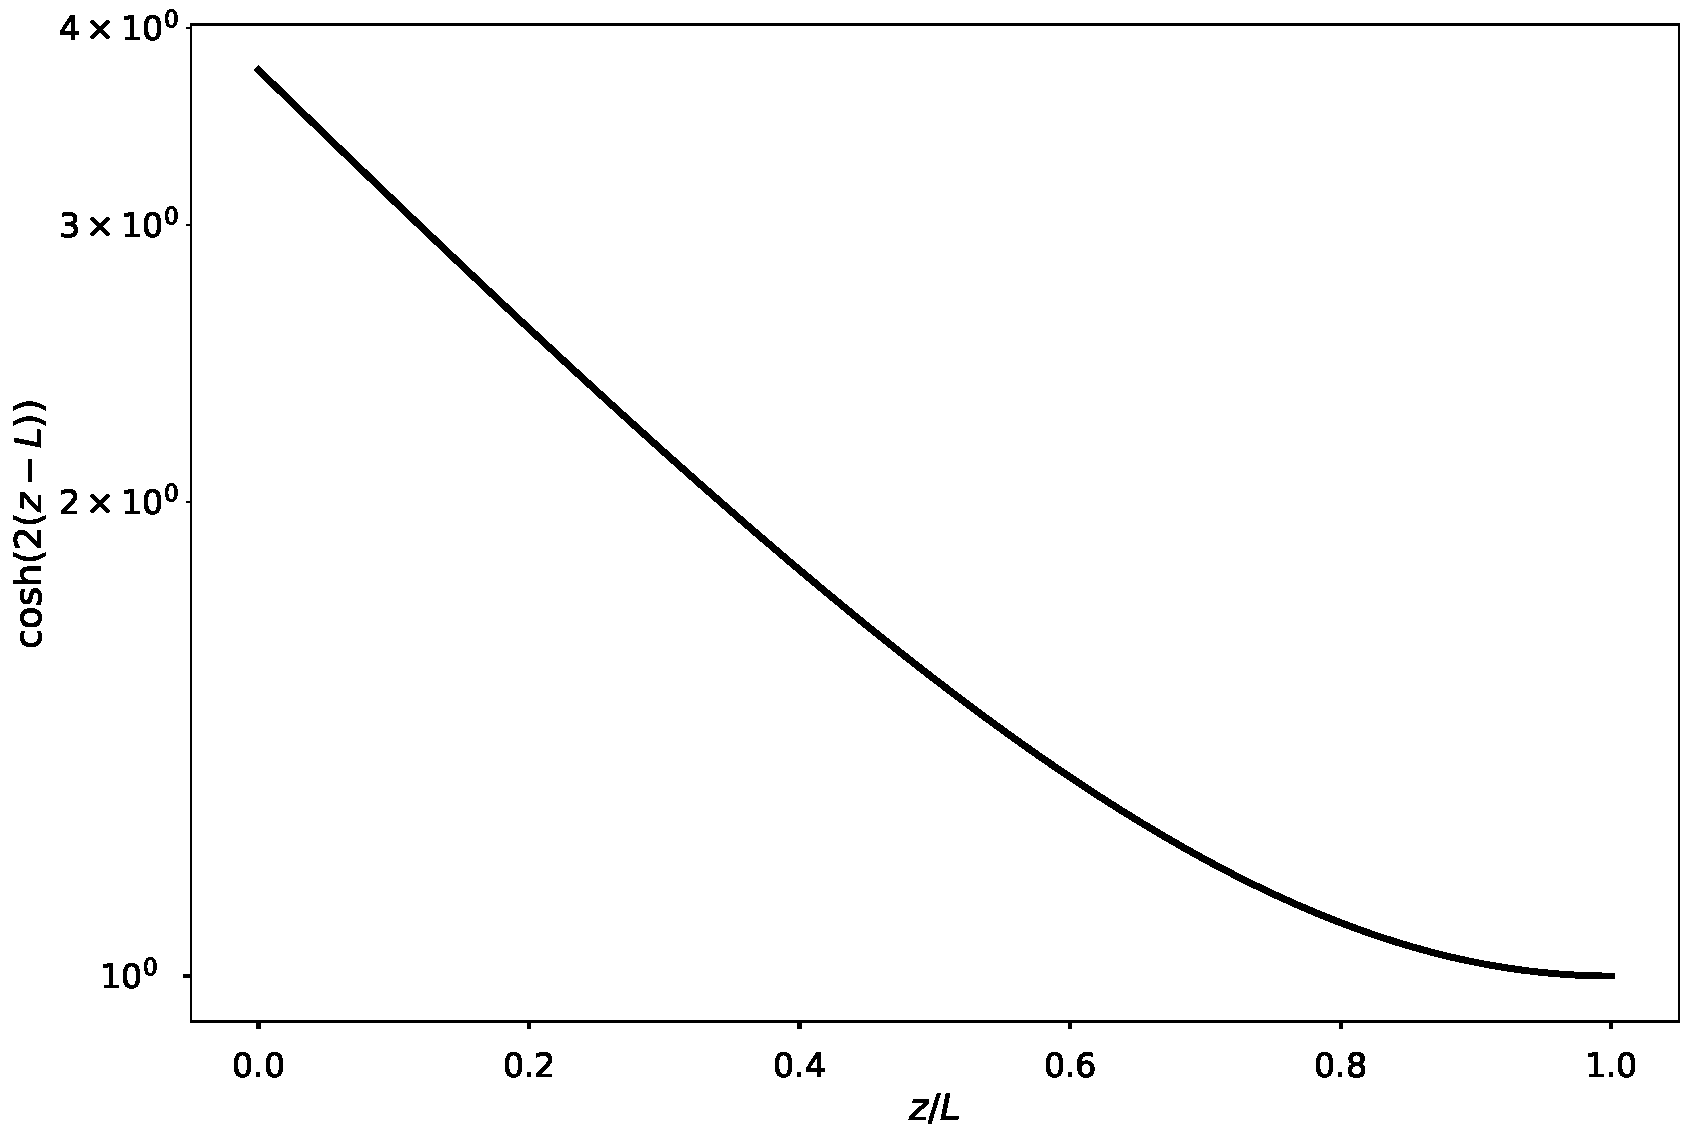
\includegraphics[width=\textwidth]{chapters/assets/halo/cosh.pdf}
%     \caption{ $\cosh(2\delta(z-L))$ with $\delta=1$ as a function of $z/L$. This function always reach the minimum at $z=L$.}
%     \label{chap:halo-sec:line-sym-fig:cosh}
% \end{figure}

\begin{figure}[htbp]
    \centering
    % 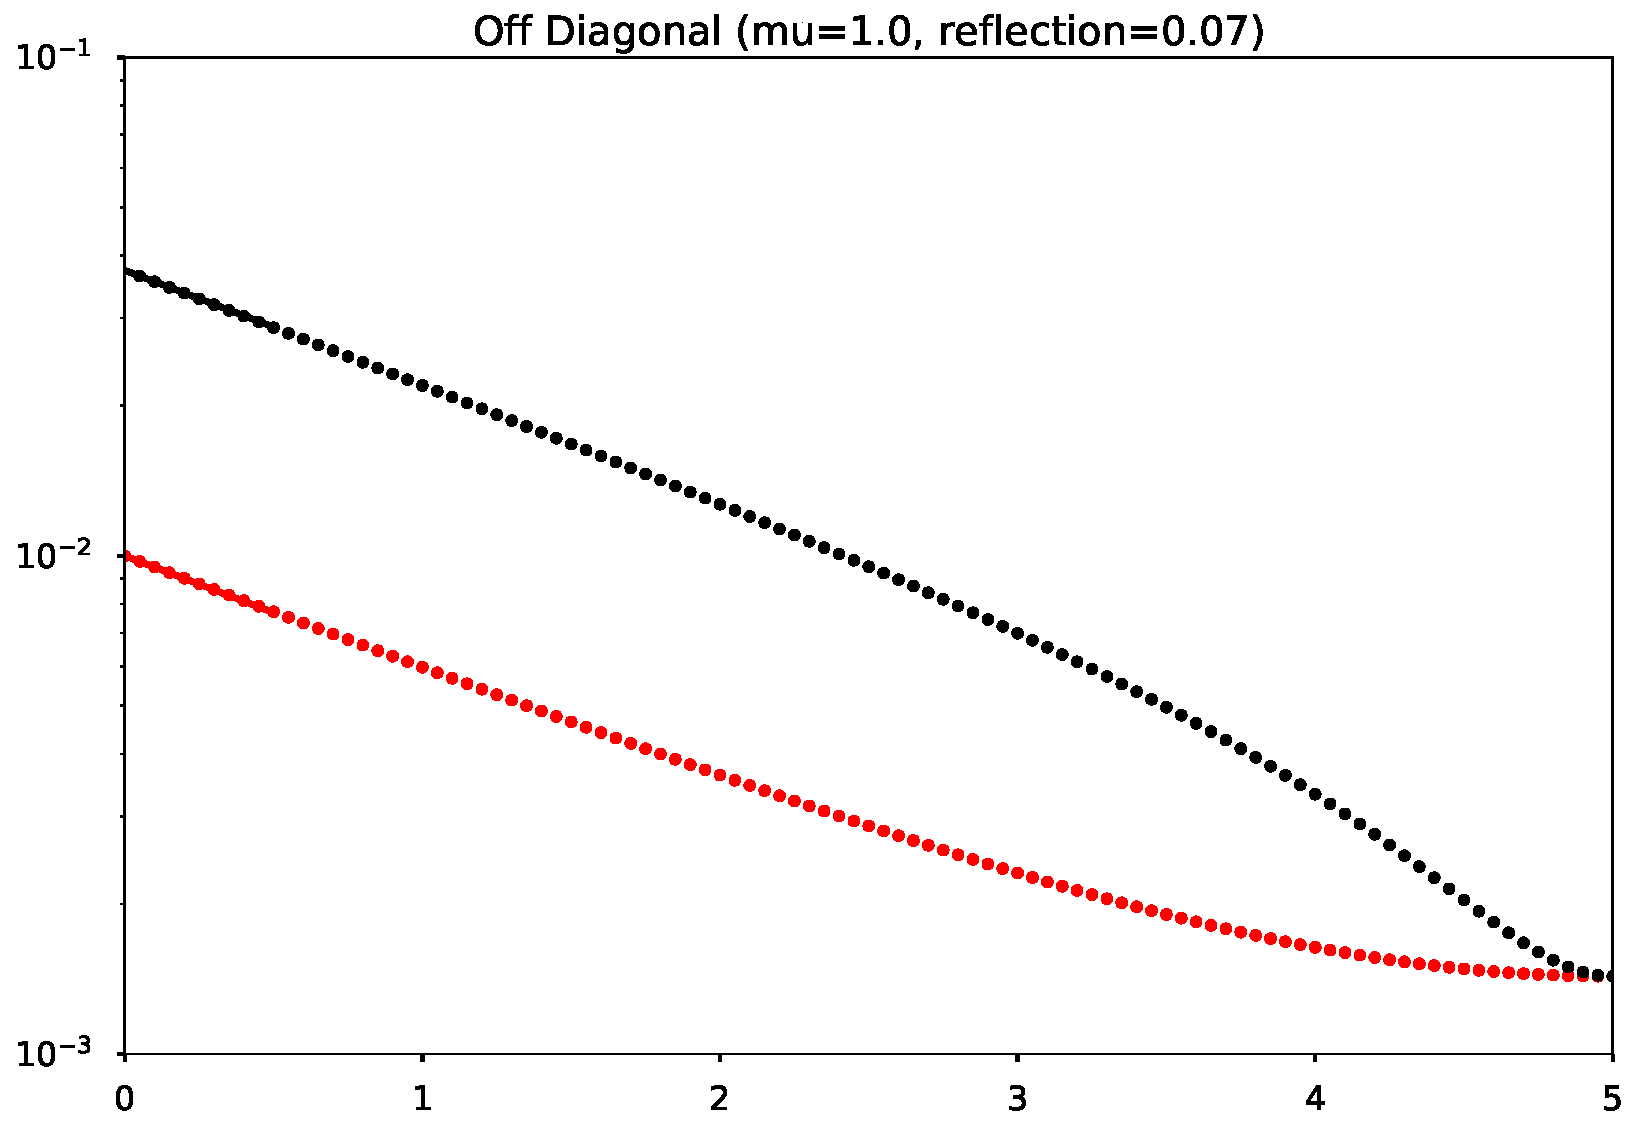
\includegraphics[width=\textwidth]{chapters/assets/halo/mu-1-reflection-0p07.pdf}
    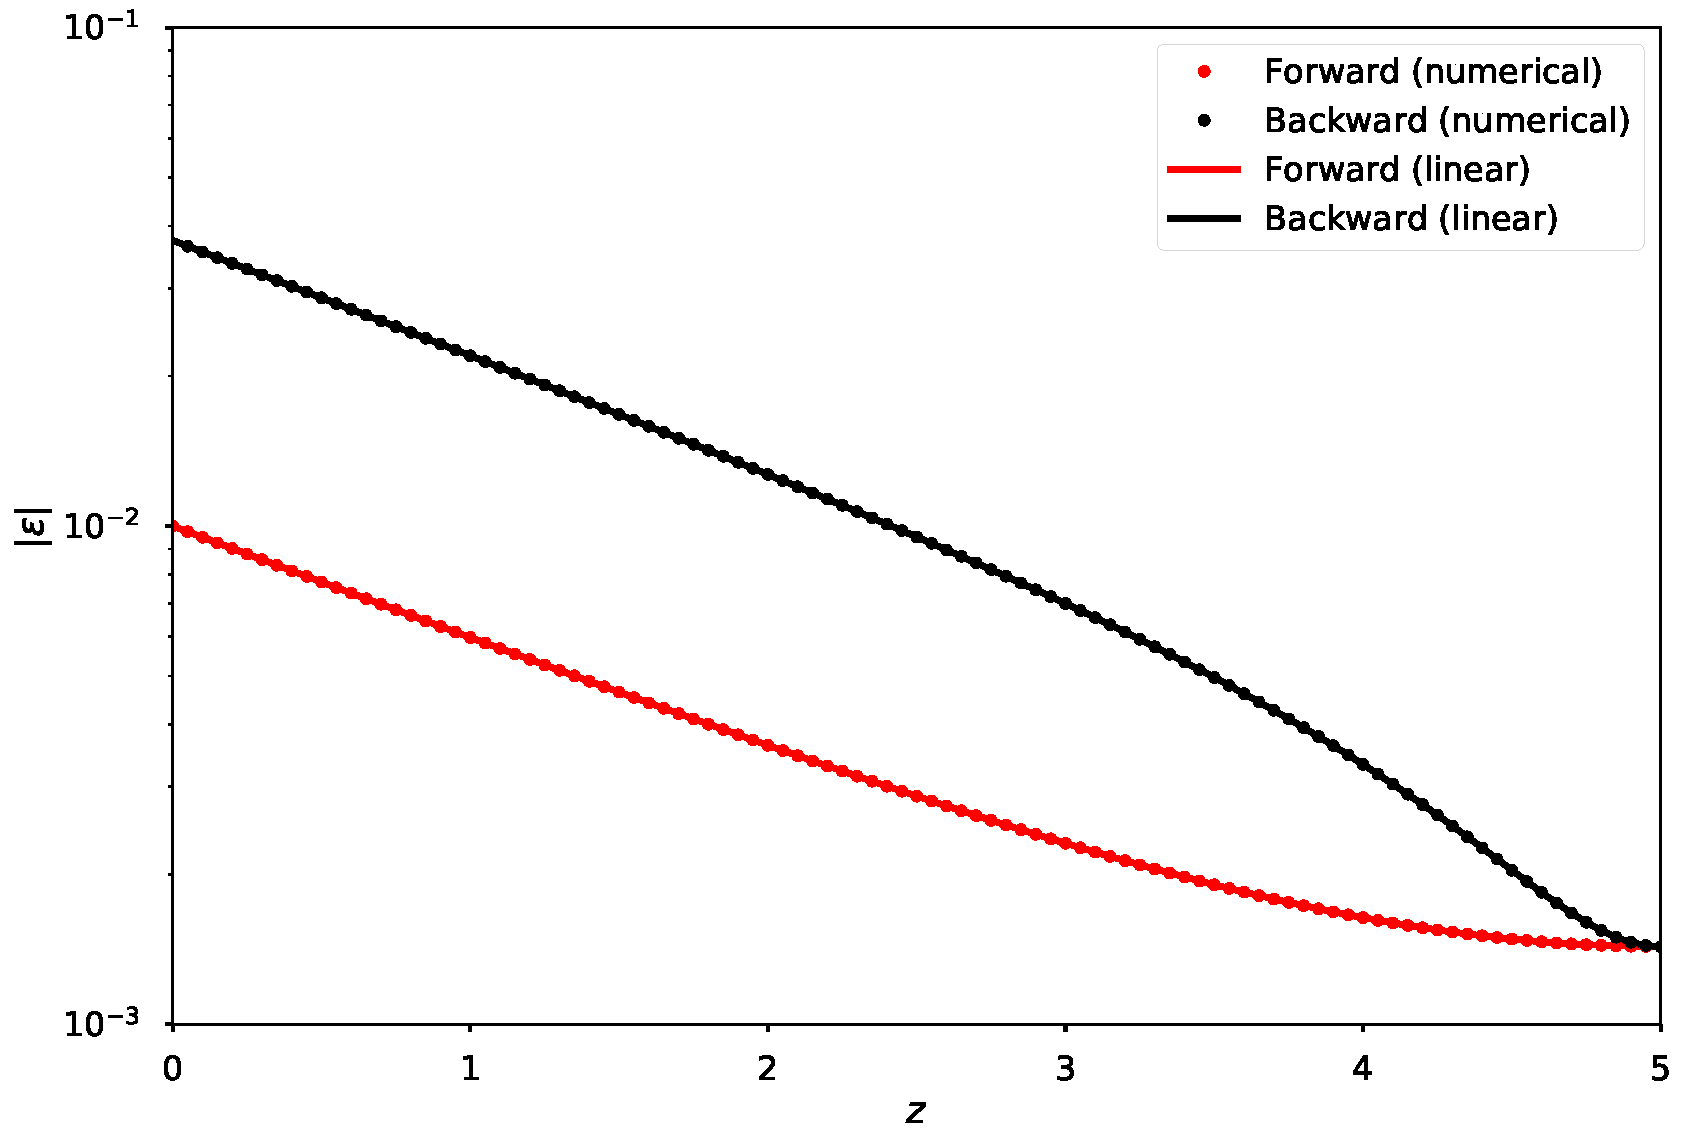
\includegraphics[width=\textwidth]{chapters/assets/halo/thesis-mu-1-refl-0p07}
    \caption{The magnitudes of the off-diagonal elements of the density matrices of the forward and reflected neutrino beams as functions of distance $z$, respectively. The markers are the numerical results for the single-beam model with $\mu'= 1.0$, $R=0.07$, $L=5/\omega_\vv$, and the normal hierarchy. The continuous curves are the analytical results obtained from Eqn.~\eqref{chap:collective-sec:halo-eqn:linearized-eom-solution}. [Change forward markers to squares, remove legends]}
    \label{chap:halo-sec:line-sym-fig:mu-1.0-reflection-0.07}
\end{figure}


For small values of $\epsilon_{\FF}$ and $\epsilon_\BB$, the solution from the linearized equation should represent the numerical calculations faithfully. In Fig.~\ref{chap:halo-sec:line-sym-fig:mu-1.0-reflection-0.07}, I plotted the numerical result (dots) as well as the result from Eqn.~\eqref{chap:collective-sec:halo-eqn:single-beam-linearized-solution} (lines). It clearly shows that the linearized solution is a great match to the numerical result. This is also a method to validate the code.





In Fig.~\ref{chap:halo-sec:line-sym-fig:mu-1.0-reflection-0.07}, I compare the numerical results obtained from the relaxation algorithm with the analytical results in Eqn.~\eqref{chap:collective-sec:halo-eqn:linearized-eom-solution} for the single-beam model with $\mu'= 1.0$, $R=0.07$, $L=5/\omega_\vv$, and the normal hierarchy. The good agreement between these results shows that the numerical code works as expected.

\begin{figure}[htbp]
    % \centering
    \minipage{0.49\textwidth}
    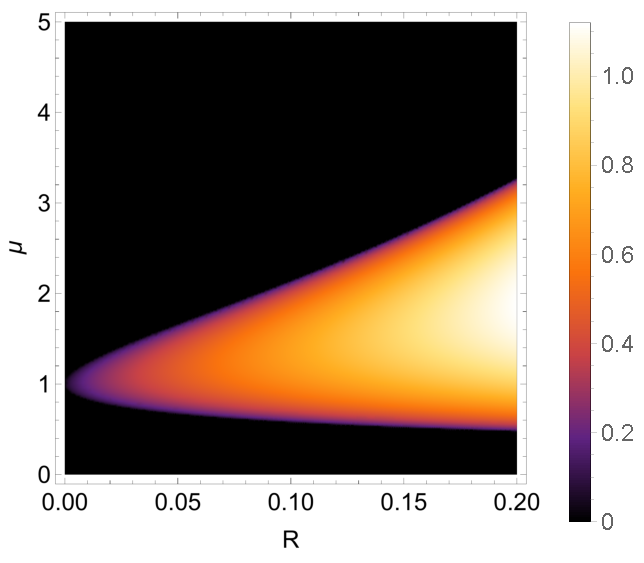
\includegraphics[width=\textwidth]{chapters/assets/halo/growth-rate-mu-refl-nh}
    \endminipage\hfill
    \minipage{0.49\textwidth}
    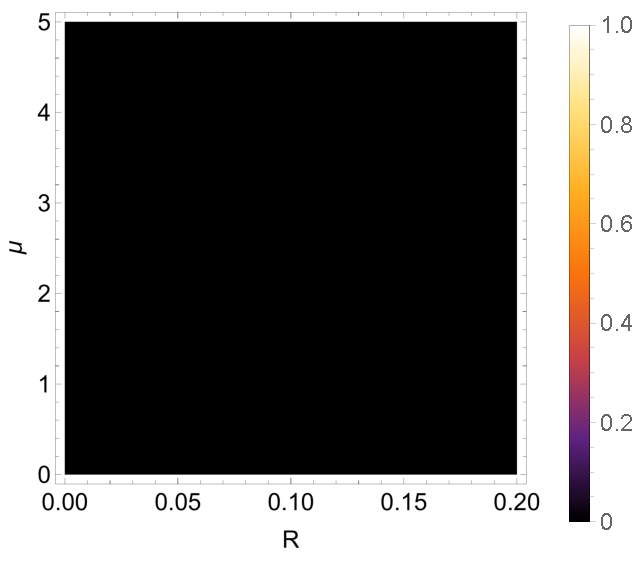
\includegraphics[width=\textwidth]{chapters/assets/halo/growth-rate-mu-refl-ih}
    \endminipage\hfill
    \caption{Instability regions for the normal hierarchy (left) and the inverted hierarchy (right) in the single-beam model with reflection. The color represents the magnitude of the imaginary component of the collective frequency.}
    \label{chap:halo-sec:line-sym-fig:instability-regions}
\end{figure}


Comparing Eqn.~\eqref{chap:collective-sec:bipolar-linearized-eom} and Eqn.~\eqref{chap:collective-sec:halo-eqn:linearized-eom-single-beam-model}, one sees that the single-beam model with reflection is equivalent to the two-beam model without reflection with the reflected neutrino beam playing the role of the antineutrino beam, $R\to \alpha$, $\eta \to -\eta$, and $\mu' \to \mu$. Therefore, there exist flavor instabilities in the single-model with reflection for the normal mass hierarchy as shown in Fig.~\ref{chap:halo-sec:line-sym-fig:instability-regions}.

% As for linear stability analysis, I will draw an analogy between this model and the bipolar model and write down the equation of motion in flavor isospin space,
% \begin{align}
%  i \partial_t \vec s_{\mathrm F} &= \vec s_{\mathrm F} \times (\vec {H}_\vv +R \mu' \vec s_{\mathrm B}) \\
%    i\partial_t \vec s_{\mathrm B} &= \vec s_{\mathrm B} \times (- \vec H_\vv - \mu' \vec s_{\mathrm F}) .
% \end{align}
% Using the result of bipolar model, I expect that only normal hierarchy has an instability region which is trivial since I noticed that the backward beam is acting like antineutrino beams but with different hierarchies. I find the instability regions in Fig.~\ref{chap:halo-sec:line-sym-fig:instability-regions}.





% \begin{figure}[htbp]
%     \centering
%     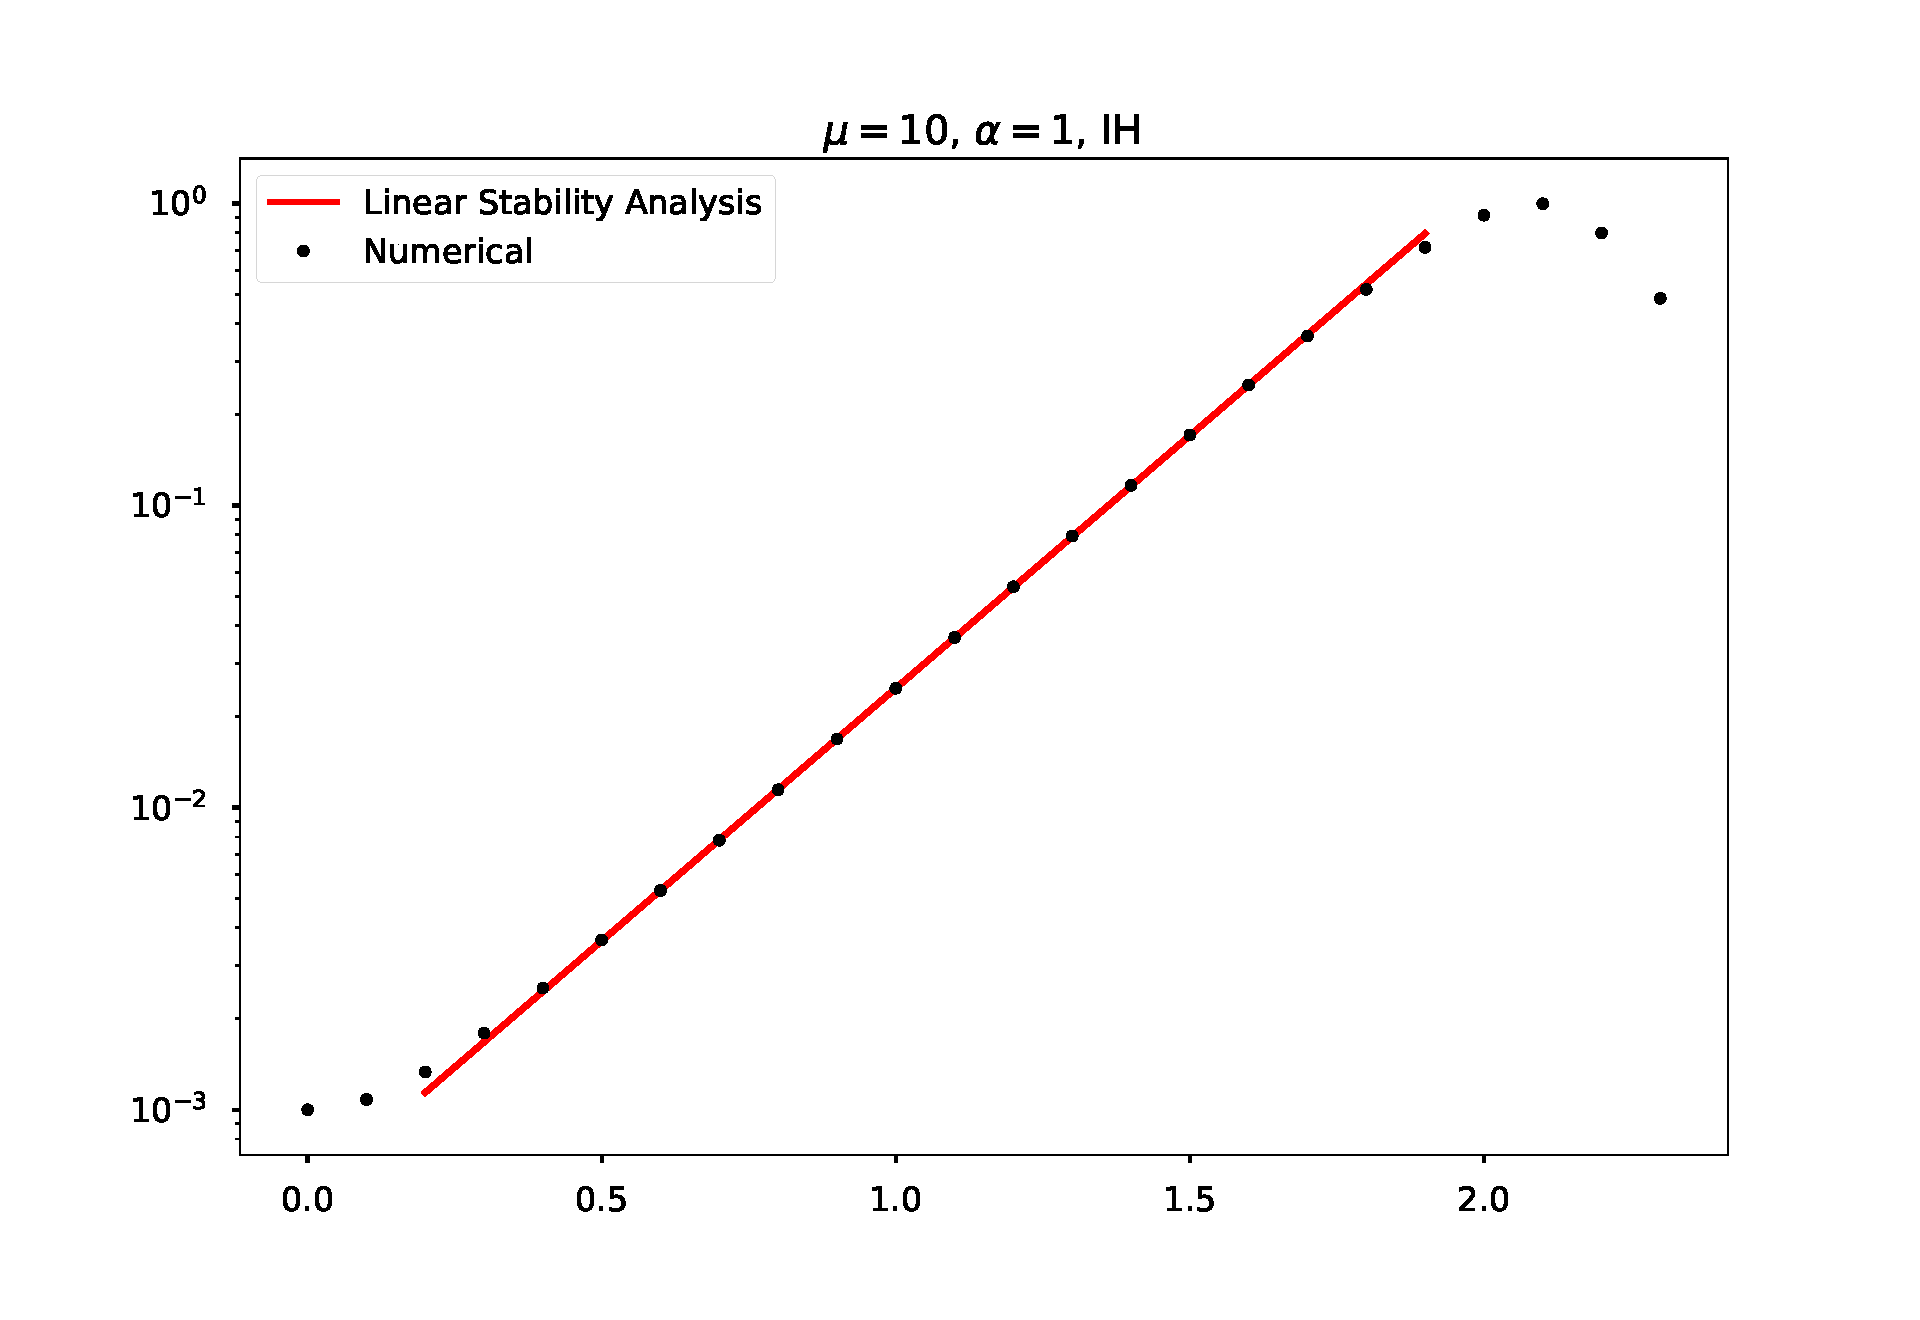
\includegraphics[width=\textwidth]{chapters/assets/halo/halo-mu-4-compare-bipolar.pdf}
%     \caption{The validation of the code by setting reflection to zero and compare with bipolar model for two beams case, where the slope is matching the theoretical value $3.85$.}
%     \label{chap:halo-sec:num-fig:compare-vac-bipolar-lsa}
% \end{figure}





%%%%%%%%%%%%%%%%%%%%%%%%%%%%%%%%%%%%%%%%%%%%%%%%%%%%%%%%%%%%%%%%%%%%%%%%%
%%%%%%%%%%%%%%%%%%%%%% Conclusion %%%%%%%%%%%%%%%%%%%%%%%%%%%%
%%%%%%%%%%%%%%%%%%%%%%%%%%%%%%%%%%%%%%%%%%%%%%%%%%%%%%%%%%%%%%%%%%%%%%%%%


\section{\label{chap:collective-sec:conclusion}Summary}

A dense neutrino medium can oscillate collectively because of the neutrino self-interaction potential. When the neutrino flavor conversion probabilities are small, one can apply the linearized flavor stability analysis to find out the regimes where neutrino oscillations begin to develop. I. Izaguirre et al. proposed that the flavor instabilities of a neutrino medium are associated with ``gaps'' between the real dispersion relation curves of the collective modes. In this chapter, I have shown that this association is not valid in general. In particular, I showed that flavor instabilities can exist in three-beam models and in models with continuous but crossed ELN distributions even without any gap in the real dispersion relation curves.

I proposed a toy model with two neutrino beams to explore neutrino oscillations with scattered fluxes such as in the supernova model with a neutrino halo. I have developed a relaxation method and a numerical code based on this method to solve the this model, and I have validated the numerical code in the scenario where only the neutrino beam and its reflected beam exist. The code can be accessed at \url{https://github.com/NeuPhysics/neutrino-halo-problem}.


% In the spirit of numerical methods, I developed a parallelable relaxation method, using C++ and OpenMP. The code is validated using vacuum oscillations and solution to the linearized equation of motion. Both the analytical and numerical results showed that for the single-beam line model is the same as the bipolar model. Thus I can perform linear stability analysis and find out the unstable regions. The reflection indeed may enhance the flavor conversions but I did not find new types of instability using the simple model. Future work should be done to explore the effect of symmetry breaking and multiple emission beams.
